\documentclass[11pt,a4paper]{article}

% ------------------------------------------------------------------ paquetes
\usepackage[utf8]{inputenc}
\usepackage[T1]{fontenc}
\usepackage{lmodern}
\usepackage[spanish,es-tabla,es-nodecimaldot]{babel}
\usepackage[margin=2.2cm]{geometry}
\usepackage{graphicx}
\usepackage{booktabs}
\usepackage{longtable}
\usepackage{float}
\usepackage{array}
\usepackage{amsmath}
\usepackage{enumitem}
\usepackage[table]{xcolor}
\usepackage[font=small,labelfont=bf,skip=4pt]{caption}
\usepackage{tcolorbox}
\usepackage{fancyhdr}
\usepackage{fancyvrb}
\usepackage[hidelinks]{hyperref}

\graphicspath{{../figures/framework/}{../figures/coach/}}
\definecolor{ame}{HTML}{1C5CAB}
\definecolor{hip}{HTML}{EB6834}
\DeclareRobustCommand{\col}[1]{\texttt{\detokenize{#1}}}
\newtcolorbox{historia}[1][]{colback=ame!5,colframe=ame,boxrule=0.6pt,arc=2pt,left=6pt,right=6pt,top=4pt,bottom=4pt,title={#1},fonttitle=\bfseries\small}
\newtcolorbox{aviso}[1][]{colback=hip!6,colframe=hip,boxrule=0.6pt,arc=2pt,left=6pt,right=6pt,top=4pt,bottom=4pt,title={#1},fonttitle=\bfseries\small}
\setlist{itemsep=2pt,topsep=3pt}
\renewcommand{\arraystretch}{1.12}
\pagestyle{fancy}\fancyhf{}
\lhead{\small ISAC Hackathon 2026 · Club América}\rhead{\small Marco analítico, variables y modelos}
\cfoot{\small\thepage}

\newcommand{\nRecursos}{1,116}
\newcommand{\mbBronze}{2,485}
\newcommand{\nEventos}{736,829}
\newcommand{\nFilasTresSesenta}{8,925,818}
\newcommand{\nLiga}{1,854}
\newcommand{\nPosesiones}{47,022}
\newcommand{\nSegmentos}{1,995}
\newcommand{\nCambios}{703}
\newcommand{\nJugPartido}{3,458}
\newcommand{\nPartidos}{222}
\newcommand{\nVarPartido}{88}
\newcommand{\rhoPPDA}{0.96}
\newcommand{\rhoPos}{0.84}
\newcommand{\rhoXG}{0.97}
\newcommand{\rhoDef}{0.71}
\newcommand{\pctTransSB}{31}
\newcommand{\ratioMin}{1.04}
\newcommand{\rhoSensMin}{0.86}
\newcommand{\nVariables}{55}
\newcommand{\nNucleo}{29}
\newcommand{\nFiabBaja}{16}
\newcommand{\nTrain}{155}
\newcommand{\nVal}{33}
\newcommand{\nTest}{34}
\newcommand{\testDesde}{2025-10-22}
\newcommand{\nTunoSupera}{8}
\newcommand{\nTuno}{12}
\newcommand{\tunoMejoraMax}{10}
\newcommand{\rivalPos}{-5.8}
\newcommand{\rivalTilt}{-9.4}
\newcommand{\localTilt}{6.2}
\newcommand{\localPress}{4.2}
\newcommand{\rivalLong}{2.0}
\newcommand{\tiltPierde}{+9.4}
\newcommand{\tiltGana}{-12.8}
\newcommand{\posPierde}{+8.4}
\newcommand{\posGana}{-5.3}
\newcommand{\tresRdos}{0.13}
\newcommand{\tresNvar}{6}
\newcommand{\cuatroAUC}{0.72}
\newcommand{\cuatroPrev}{12}
\newcommand{\pcUnoVar}{38}
\newcommand{\nPC}{5}
\newcommand{\tipoUnoPos}{58}
\newcommand{\tipoDosPos}{46}
\newcommand{\tipoUnoTilt}{69}
\newcommand{\tipoDosTilt}{44}
\newcommand{\tipoUnoPPDA}{11.7}
\newcommand{\tipoDosPPDA}{18.5}
\newcommand{\silDos}{0.26}
\newcommand{\nRoles}{5}
\newcommand{\silRoles}{0.12}
\newcommand{\nCards}{33}
\newcommand{\nSupervisados}{31}
\newcommand{\nSupera}{20}
\newcommand{\medTopTres}{62}
\newcommand{\medTopUno}{28}
\newcommand{\medBoost}{45}
\newcommand{\medShareDef}{35}
\newcommand{\medShareMid}{25}
\newcommand{\medShareFwd}{3}
\newcommand{\medShareWide}{17}
\newcommand{\medGiniTouch}{0.35}


\title{\textbf{Del dato al criterio}\\[4pt]
\large Pipeline medallion, marco analítico, formulación de modelos y ficha automática por partido\\[2pt]
\normalsize Reto ISAC 2026: \emph{La historia de un entrenador a través de los datos} --- Fase 2}
\author{Equipo ISAC-Hackathon-America}
\date{Septiembre de 2026}

\begin{document}
\maketitle
\thispagestyle{empty}

\begin{abstract}
\noindent El análisis exploratorio (fase 1) describió los datos. Esta segunda fase construye la infraestructura y el
método para responder la pregunta del reto con el \textbf{partido como unidad de estudio}. Primero, un \emph{pipeline}
local con arquitectura \emph{medallion} (Bronze $\rightarrow$ Silver $\rightarrow$ Gold, en Parquet) extrae \nRecursos{}
recursos de la API de StatsBomb, los valida con compuertas de calidad y reproduce exactamente los datos del EDA.
Segundo, un \textbf{marco analítico} explícito define cada objeto táctico; se valida contra StatsBomb (PPDA
$\rho=\rhoPPDA$, np xG $\rho=\rhoXG$) y es robusto a sus umbrales ($\rho\geq\rhoSensMin$). Tercero, \nVariables{}
variables por partido, incluida una dimensión nueva sobre \emph{cómo se reparte el juego entre los jugadores}, se evalúan
como criterios medibles (fiabilidad, discriminación, estabilidad, sensibilidad, redundancia y validez) y se reducen a
\nNucleo{} variables núcleo. Cuarto, siguiendo el ciclo de vida del aprendizaje supervisado, se formulan once tareas
(T1--T7 supervisadas, U1--U3 no supervisadas), cada una con su $y$, $x$, partición temporal, baseline y métrica.
Los modelos base superan a su baseline en \nSupera{} de \nSupervisados{} casos; sus fracasos también informan. Por
último, todo se integra en un producto: una \textbf{ficha HTML automática por partido} con el partido actual, la
comparación histórica y una proyección, trazable a \emph{model cards} y con monitoreo de \emph{drift}.
\par\smallskip\noindent\textbf{ADN del entrenador.} Con las estadísticas de los 1,789 partidos de la liga se perfila a
los \nTecnicos{} técnicos de la Liga MX en 8 rasgos de juego, ajustados por rival y localía. Con la partición oficial
(entrenamiento 2021--2025, prueba 2026), el ADN reconoce a Almada en el América sin haberlo visto nunca ahí (posición
mediana \almadaRank{} de 31): el estilo sigue al técnico. Es la base de un producto para contratar, dar seguimiento y
preparar partidos, con escenarios de ROI.
\end{abstract}

\tableofcontents
\newpage

% =====================================================================
\section{Definición del problema}\label{sec:problema}
% =====================================================================
\begin{historia}[Pregunta central del reto]
¿Cuáles son los principios que definen al equipo en fase ofensiva y defensiva, cómo se manifiestan estos patrones a lo
largo del tiempo, y de qué manera se ajusta el comportamiento en función del contexto del partido (rival, marcador,
localía o momento del juego)?
\end{historia}

\paragraph{Necesidad.} Que alguien que no vio los partidos entienda el estilo del equipo, sus ideas, cómo usa a sus
jugadores y cómo todo eso se repite, evoluciona y se ajusta.

\paragraph{Unidad de estudio.} El \textbf{partido}, junto con sus derivados: la posesión, el tramo de 15 minutos con su
estado del marcador, la jugada a balón parado, la intervención de cambios y el jugador dentro de un partido. El
entrenador \textbf{no} es una variable del modelo. Se conserva como metadato (\col{team_manager}) para particiones
posteriores, de modo que las conclusiones se construyen sobre el comportamiento observado y no sobre etiquetas.

\paragraph{Formulación global.} Siguiendo la definición de Mitchell (T/E/P):
\begin{itemize}
  \item \textbf{T (tarea):} describir, explicar y anticipar el comportamiento del equipo por partido.
  \item \textbf{E (experiencia):} \nPartidos{} partidos de Liga MX (julio 2021 -- septiembre 2026) con eventos StatsBomb y
        StatsBomb 360.
  \item \textbf{P (desempeño):} error de generalización en una \emph{prueba temporal} (los partidos más recientes) frente
        a un baseline, e interpretabilidad trazable al marco analítico.
\end{itemize}
La pregunta se descompone en tareas concretas (Tabla~\ref{tab:tareas}). Cada una tiene su variable objetivo, sus
variables explicativas y su métrica. Las tareas supervisadas explican o anticipan; las no supervisadas descubren
estructura (ejes de estilo, tipos de partido y roles de jugador).

\begin{table}[H]
\centering
\scriptsize
\caption{Formulación de las tareas: variable objetivo ($y$), explicativas ($x$), tipo de problema, modelos (del baseline a los candidatos) y medida de desempeño ($P$).}
\label{tab:tareas}
\resizebox{\ifdim\width>\linewidth\linewidth\else\width\fi}{!}{%
\begin{tabular}{l p{2.1cm} p{0.9cm} p{1.8cm} p{2.1cm} p{3.2cm} p{1.5cm} p{2.6cm} p{1.5cm}}
\toprule
\textbf{tarea} & \textbf{nombre} & \textbf{reto} & \textbf{unidad (Gold)} & \textbf{y} & \textbf{x} & \textbf{tipo} & \textbf{modelos} & \textbf{P} \\
\midrule
T1 & Ajuste al contexto previo & 5.2 & match\_features + dim\_match & 12 variables de estilo & localía, fuerza del rival previa, fase, descanso, orden, inercia (5 previos) & Regresión & Baseline $\rightarrow$ Ridge / LASSO $\rightarrow$ Árbol $\rightarrow$ KNN & MAE, RMSE, R$^2$ \\
T2 & Ajuste intra-partido & 5.2 & fct\_segment & estilo en el tramo & estado del marcador, tramo de 15', localía, fase, fuerza del rival & Regresión & Baseline $\rightarrow$ Ridge $\rightarrow$ Árbol & MAE, R$^2$ \\
T3 & Principios que generan dominio & 5.1, 5.5 & match\_features & OBV neto, diferencial np xG & 24 métricas de proceso (sin resultado) & Regresión & Baseline $\rightarrow$ LASSO (+bootstrap) $\rightarrow$ Árbol $\rightarrow$ KNN & MAE, RMSE, R$^2$ \\
T3b & Resultado & 5.5 & match\_features & G / E / P & 24 métricas de proceso & Multiclase & Clase mayoritaria $\rightarrow$ Logística softmax $\rightarrow$ Árbol & F1 macro, exactitud, matriz de confusión \\
T4 & Posesión $\rightarrow$ ocasión & 5.1 & fct\_possession & la posesión termina en tiro & inicio (x, y), patrón, recuperación, marcador, minuto, localía, rival & Binaria desbalanceada & Tasa base $\rightarrow$ Logística $\rightarrow$ Árbol $\rightarrow$ KNN & ROC-AUC, F1, Brier \\
T5 & Balón parado & 5.4 & fct\_set\_piece & el balón parado termina en tiro & tipo, entrega, zona de destino, lado, altura & Binaria & Tasa base $\rightarrow$ Logística $\rightarrow$ Árbol & ROC-AUC, Brier \\
T6 & Impacto de sustituciones & 5.3 & fct\_substitution & $\Delta$ OBV neto, $\Delta$ field tilt, $\Delta$ np xG (15' después -- antes) & minuto, marcador, n.º de cambios, líneas que salen, localía, rival & Regresión & $\Delta$=0 / $\Delta$ medio $\rightarrow$ Ridge $\rightarrow$ Árbol & MAE, R$^2$ \\
T7 & Distribución del juego & 5.3, 5.2 & match\_features & Gini de toques/progresión, top-3 OBV, potenciación & contexto previo + inercia & Regresión & Baseline $\rightarrow$ Ridge / LASSO $\rightarrow$ Árbol $\rightarrow$ KNN & MAE, R$^2$ \\
U1 & Ejes de estilo & 5.1, 5.2 & match\_features & — & 12 variables de estilo & Reducción de dimensión & PCA (70 \% varianza) & varianza explicada \\
U2 & Tipos de partido & 5.2 & componentes U1 & — & — & Clustering & K-means (k por silhouette) & silhouette \\
U3 & Roles de jugador & 5.3 & fct\_player\_match ($\geq$30') & — & 14 acciones p90 & Clustering & K-means (k por silhouette) & silhouette, interpretabilidad \\
\bottomrule
\end{tabular}}
\end{table}

% =====================================================================
\section{Arquitectura de datos y pipeline}\label{sec:pipeline}
% =====================================================================
\subsection{Capas medallion}
Los datos se organizan en tres capas, todas locales y en Parquet (formato columnar comprimido que se lee más rápido y
conserva los tipos). No se usa nube ni motores SQL: el volumen (unos 2.5 GB crudos) cabe en memoria y pandas basta.

\begin{center}
\small
\begin{tabular}{p{2.2cm} p{5.6cm} p{6.6cm}}
\toprule
\textbf{Capa} & \textbf{Contenido} & \textbf{Reglas} \\
\midrule
\textbf{Bronze} & Respuesta \emph{exacta} de la API (\texttt{.json.gz}) por endpoint y partido, más el calendario de toda la liga. & Inmutable. Manifest con URL, versión, fecha de extracción, status, bytes y sha256. Incremental: salta lo ya extraído. \\
\textbf{Silver} & Una tabla Parquet por entidad: partidos, liga, eventos y 360 (particionados por temporada), alineaciones, estadísticas de jugador y equipo. & Aplanado idéntico al de \texttt{statsbombpy}, leyendo de Bronze sin red. Compuertas de calidad: si una falla, el pipeline se detiene. \\
\textbf{Gold} & Tablas por caso de uso: contexto sin \emph{leakage}, posesiones, tramos, balón parado, cambios, jugador $\times$ partido y variables por partido. & Se reconstruye completo desde Silver con las definiciones del marco. Cambiar una definición solo requiere volver a correr Gold. \\
\bottomrule
\end{tabular}
\end{center}

El pipeline se ejecuta con un solo comando y cada etapa lee únicamente de la anterior:
\begin{center}
\texttt{python -m src.pipeline run -{}-stages bronze,silver,gold,train,score,report [-{}-match-id \dots]}
\end{center}

\begin{table}[H]
\centering
\small
\caption{Capa Bronze: recursos extraídos por endpoint (manifest).}
\label{tab:bronze}
\resizebox{\ifdim\width>\linewidth\linewidth\else\width\fi}{!}{%
\begin{tabular}{lrrrr}
\toprule
\textbf{endpoint} & \textbf{recursos} & \textbf{MB} & \textbf{\% status 200} & \textbf{respuestas vacías} \\
\midrule
360-frames & 222 & 1,195 & 100 & 1 \\
events & 222 & 1,235 & 100 & 0 \\
lineups & 222 & 6.3 & 100 & 0 \\
matches & 6 & 2.7 & 100 & 0 \\
player-match-stats & 222 & 42.6 & 100 & 0 \\
team-match-stats & 222 & 3.5 & 100 & 0 \\
\bottomrule
\end{tabular}}
\end{table}
\begin{table}[H]
\centering
\small
\caption{Capa Silver: tablas Parquet (para \texttt{events} y \texttt{frames360}, filas totales y número de particiones por temporada).}
\label{tab:silver}
\resizebox{\ifdim\width>\linewidth\linewidth\else\width\fi}{!}{%
\begin{tabular}{lrr}
\toprule
\textbf{tabla} & \textbf{filas} & \textbf{columnas / particiones} \\
\midrule
league\_matches & 1,854 & 62 \\
league\_team\_match\_stats & 3,578 & 218 \\
lineup\_positions & 9,699 & 14 \\
lineups & 9,317 & 16 \\
matches & 230 & 70 \\
player\_match\_stats & 6,870 & 178 \\
team\_match\_stats & 444 & 208 \\
events & 736,829 & 6 \\
frames360 & 8,925,818 & 6 \\
\bottomrule
\end{tabular}}
\end{table}
\begin{table}[H]
\centering
\small
\caption{Capa Gold: tablas por caso de uso.}
\label{tab:gold}
\resizebox{\ifdim\width>\linewidth\linewidth\else\width\fi}{!}{%
\begin{tabular}{lrr}
\toprule
\textbf{tabla} & \textbf{filas} & \textbf{columnas} \\
\midrule
dim\_coach & 149 & 7 \\
dim\_match & 222 & 18 \\
fct\_player\_match & 3,458 & 44 \\
fct\_possession & 47,022 & 32 \\
fct\_segment & 1,995 & 50 \\
fct\_set\_piece & 12,509 & 48 \\
fct\_substitution & 703 & 25 \\
fct\_team\_match\_league & 3,578 & 221 \\
match\_features & 222 & 88 \\
\bottomrule
\end{tabular}}
\end{table}

\subsection{Compuertas de calidad, idempotencia y linaje}
Silver valida, por temporada: que los eventos cubren todos los partidos jugados, que los identificadores son únicos,
que las coordenadas caen dentro de la cancha de $120\times80$, que todo tiro tiene xG y que cada partido tiene dos
alineaciones iniciales. Al final valida que el \textbf{marcador reconstruido desde eventos coincide con el oficial en
el 100\,\% de los partidos}, que cada partido tiene dos filas de estadísticas de equipo y que la precisión de pase
corregida está en rango. Esta última corrige una anomalía detectada en el EDA: la columna de la API
\col{team_match_passing_ratio} es idéntica a \col{opp_final_third_pass_ratio}.

\begin{itemize}
  \item \textbf{Idempotencia}: una segunda corrida de Bronze descarga 0 recursos y Silver/Gold se sobrescriben
        completos. Ante cortes de red, Bronze reintenta con espera exponencial; lo que aún falle queda registrado en el
        manifest y se reintenta en la siguiente corrida.
  \item \textbf{Migración verificada}: Silver reproduce exactamente los datos del EDA (los mismos \nEventos{} eventos e
        identificadores y las mismas sumas de xG y OBV), así que los hallazgos de la fase 1 siguen siendo válidos.
  \item \textbf{Linaje}: cada \emph{model card} guarda el \emph{hash} de la tabla Gold con la que se entrenó
        (Sección~\ref{sec:implementacion}).
\end{itemize}

% =====================================================================
\section{Marco analítico}\label{sec:marco}
% =====================================================================
El módulo \texttt{src/framework.py} es la \textbf{fuente única} de definiciones (reto 5.6). Gold, los modelos, las
gráficas y la ficha lo importan; ningún notebook redefine un objeto.

\begin{itemize}
  \item \textbf{Posesión}: la de StatsBomb. \textbf{Secuencia ofensiva}: al menos 3 pases o llegada a $x\geq80$.
  \item \textbf{Zonas}: tercios (40/80), carriles (tercios de ancho), área y zona de peligro.
  \item \textbf{Fases}: construcción (la posesión nace en $x<40$ en juego abierto), progresión (cruza de $x<60$ a
        $x\geq80$) y finalización.
  \item \textbf{Transición ofensiva}: posesión que nace de una recuperación y llega a $x\geq80$ o termina en tiro en
        $\leq15$\,s. \textbf{Transición defensiva}: los 5\,s posteriores a una pérdida en juego.
  \item \textbf{Presión}: alta ($x\geq60$), media (40--60) y baja; \textbf{PPDA} propio: pases rivales de juego abierto
        en su 60\,\% propio ($x\leq72$) entre entradas, intercepciones y faltas propias en nuestro 60\,\% alto
        ($x\geq48$).
  \item \textbf{Balón parado}: córner, tiro libre y saque de banda en $x\geq80$. \textbf{Estado del marcador}: 5 niveles,
        calculado \emph{antes} de cada evento. \textbf{Tramos} de 15'. \textbf{Grupos de posición}: portero, defensas,
        carrileros, medios defensivos, medios, medios ofensivos, bandas y delanteros.
\end{itemize}
Todos los umbrales están en \texttt{ASSUMPTIONS} (Apéndice~\ref{app:assumptions}).

\subsection{Validación del marco}
Una definición propia solo es útil si mide lo que dice medir. Donde existe una métrica comparable de StatsBomb, se
compara el \emph{orden} de los partidos (Tabla~\ref{tab:validations}).

\begin{table}[H]
\centering
\small
\caption{Validación del marco analítico contra StatsBomb y contra datos oficiales.}
\label{tab:validations}
\resizebox{\ifdim\width>\linewidth\linewidth\else\width\fi}{!}{%
\begin{tabular}{p{8.5cm}rrc}
\toprule
\textbf{validación} & \textbf{valor} & \textbf{criterio} & \textbf{cumple} \\
\midrule
Transición ofensiva (propia) marcada también por StatsBomb (\%) & 100.000 & $\geq$ 70 & sí \\
Posesiones is\_transition de StatsBomb detectadas por la definición propia (\%) & 31.139 & informativo & -- \\
PPDA propio vs PPDA StatsBomb ($\rho$ Spearman) & 0.959 & > 0.8 & sí \\
Posesión (tiempo) vs posesión StatsBomb ($\rho$) & 0.836 & > 0.8 & sí \\
np xG/100 pos. vs np xG StatsBomb ($\rho$) & 0.971 & > 0.8 & sí \\
Altura acciones def. vs defensive distance SB ($\rho$) & 0.714 & > 0.6 & sí \\
Marcador reconstruido == oficial (\% partidos) & 100.000 & = 100 & sí \\
Minutos fct\_player\_match / minutos por alineaciones (mediana) & 1.042 & $\approx$ 1 & sí \\
\bottomrule
\end{tabular}}
\end{table}

\begin{itemize}
  \item El PPDA propio ordena los partidos casi igual que el de StatsBomb ($\rho=\rhoPPDA$). Se llegó a esa definición
        probando 16 variantes (4 conjuntos de acciones por 4 zonas).
  \item Todas las transiciones propias las marca también StatsBomb, pero la definición propia solo captura el
        \pctTransSB\,\% de las suyas. Es deliberado: \col{is_transition} marca cualquier posesión que nace de una
        recuperación, mientras que aquí se exige que la transición sea \emph{efectiva}.
  \item Los minutos por jugador (StatsBomb) cuadran con los que se reconstruyen desde las alineaciones (razón
        \ratioMin); la pequeña diferencia viene del tiempo añadido.
\end{itemize}

\subsection{Sensibilidad de los umbrales}
Si mover un umbral cambiara qué partidos se ven como "más presionantes" o "más verticales", las conclusiones dependerían
de una elección arbitraria. La Tabla~\ref{tab:sensitivity} recalcula tres métricas con valores alternativos:
cambia el \emph{nivel}, pero el \emph{orden} de los partidos se conserva ($\rho\geq\rhoSensMin$).

\begin{table}[H]
\centering
\small
\caption{Sensibilidad de las métricas a los umbrales: nivel medio y correlación de Spearman del ranking de partidos con la versión base.}
\label{tab:sensitivity}
\resizebox{\ifdim\width>\linewidth\linewidth\else\width\fi}{!}{%
\begin{tabular}{lrrrr}
\toprule
\textbf{supuesto} & \textbf{valor} & \textbf{métrica} & \textbf{media} & \textbf{$\rho$ vs base} \\
\midrule
transition\_window\_s & 10.000 & transition\_poss\_pct & 13.994 & 0.905 \\
transition\_window\_s (base) & 15.000 & transition\_poss\_pct & 17.791 & 1.000 \\
transition\_window\_s & 20.000 & transition\_poss\_pct & 19.928 & 0.960 \\
press\_high\_x & 55.000 & high\_press\_pct & 47.094 & 0.976 \\
press\_high\_x (base) & 60.000 & high\_press\_pct & 41.984 & 1.000 \\
press\_high\_x & 65.000 & high\_press\_pct & 36.889 & 0.978 \\
progressive\_min\_gain & 0.200 & prog\_passes\_per100 & 9.745 & 0.861 \\
progressive\_min\_gain (base) & 0.250 & prog\_passes\_per100 & 6.946 & 1.000 \\
progressive\_min\_gain & 0.300 & prog\_passes\_per100 & 4.993 & 0.893 \\
\bottomrule
\end{tabular}}
\end{table}

% =====================================================================
\section{Ingeniería y evaluación de variables}\label{sec:variables}
% =====================================================================
\subsection{Variables por criterio}
Se construyen \nVariables{} variables por partido, agrupadas por los criterios del reto: construcción, progresión,
ocasiones, presión, organización defensiva, transiciones, dominio, balón parado y uso de jugadores (catálogo completo en
el Apéndice~\ref{app:catalog}). Tres decisiones de diseño:
\begin{enumerate}
  \item \textbf{Tasas, no conteos.} Un conteo depende de la duración y del ritmo del partido; una tasa (por 100 pases,
        por 100 posesiones o en porcentaje) es comparable entre partidos.
  \item \textbf{Una sola función de agregación.} \texttt{features.aggregate(ev, poss, keys)} calcula las mismas métricas
        para cualquier agrupación: partido, mitad, tramo con estado del marcador o ventana alrededor de un cambio. Así
        el partido y sus segmentos usan exactamente las mismas definiciones.
  \item \textbf{Versión del rival.} Las métricas defensivas miden lo que el rival logra contra el equipo.
\end{enumerate}

\subsection{Uso de jugadores y distribución del juego (5.3)}
La dimensión de jugadores se pregunta si una sola posición o un solo jugador "brilla", o si el juego está repartido,
y si el sistema potencia a cada jugador. Desde \col{fct_player_match} (\nJugPartido{} filas jugador $\times$ partido)
se agregan al partido:
\begin{itemize}
  \item \textbf{Concentración}: índice de Gini del OBV, de los toques y de las acciones progresivas (0 = reparto
        perfecto; 1 = todo en un jugador).
  \item \textbf{Dependencia}: porcentaje del OBV positivo que generan el mejor jugador y los tres mejores.
  \item \textbf{Reparto por línea}: porcentaje del OBV positivo por defensas y carrileros, medios, bandas y delanteros.
  \item \textbf{Potenciación}: el OBV por 90' de cada jugador se compara con \emph{su propia} referencia previa (la media
        de sus 10 partidos anteriores, con \texttt{shift(1)} para no usar el partido actual). Se reporta el porcentaje de
        jugadores por encima de su referencia y el residuo medio.
  \item \textbf{Rotación y ajustes}: cambios en el XI respecto al partido anterior, cambios de sistema y minuto del
        primer cambio.
\end{itemize}

\begin{figure}[H]
\centering
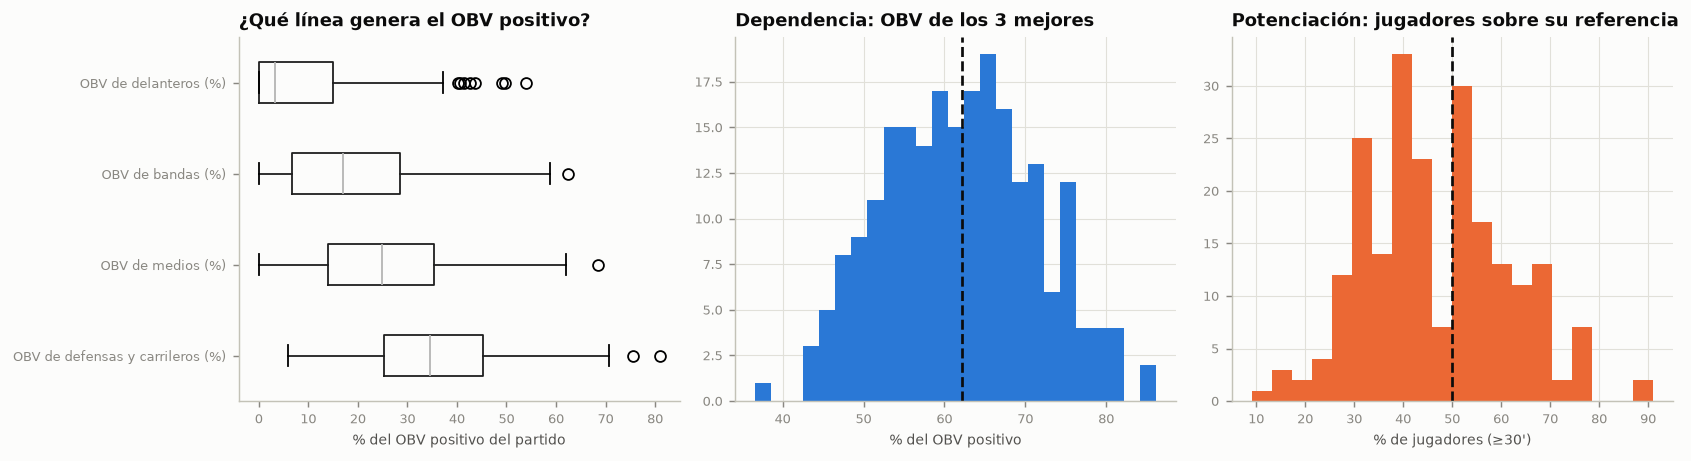
\includegraphics[width=\linewidth]{players_distribution.png}
\caption{Distribución del juego entre jugadores: reparto del OBV positivo por línea, dependencia de los tres mejores y
porcentaje de jugadores que rinden por encima de su referencia previa.}
\label{fig:players}
\end{figure}

\begin{historia}[Lo que muestran los datos: el juego está repartido y se construye desde atrás]
\begin{itemize}
  \item En el partido mediano, los tres mejores jugadores generan el \medTopTres\,\% del OBV positivo y el mejor el
        \medTopUno\,\%: hay protagonistas, pero ningún partido depende de uno solo.
  \item Por línea, defensas y carrileros generan el \medShareDef\,\% del OBV positivo, los medios el \medShareMid\,\%, las
        bandas el \medShareWide\,\% y los delanteros apenas el \medShareFwd\,\% (medianas). El valor se construye desde
        atrás y por fuera.
  \item En el partido mediano, el \medBoost\,\% de los jugadores rinde por encima de su propia referencia previa. Que sea
        algo menos de la mitad es lo esperable por regresión a la media, así que la potenciación debe leerse partido a
        partido, no como promedio.
\end{itemize}
\end{historia}

\subsection{Evaluación de las variables como criterios}
Una métrica solo sirve como criterio si mide algo \emph{del partido} y no ruido. Cada variable se evalúa en seis
dimensiones:
\begin{enumerate}
  \item \textbf{Fiabilidad intra-partido}: la correlación entre su valor en el primer y en el segundo tiempo, corregida
        con Spearman-Brown al partido completo.
  \item \textbf{Discriminación}: ICC(1), tratando los dos tiempos como mediciones repetidas del mismo partido.
  \item \textbf{Estabilidad temporal}: autocorrelación lag-1 entre partidos consecutivos.
  \item \textbf{Sensibilidad al contexto}: $R^2$ de localía, fuerza del rival y fase.
  \item \textbf{Redundancia}: máximo $|\rho|$ con otra variable y VIF; se liga al supuesto de no multicolinealidad.
  \item \textbf{Validez}: correlación con el diferencial de np xG y con el OBV neto.
\end{enumerate}

\paragraph{Selección del núcleo.} Las reglas, en orden:
\begin{enumerate}
  \item Se excluyen las variables de resultado (OBV neto y diferencial de xG): son objetivos, no criterios de estilo.
  \item Se exige una fiabilidad $\geq0.30$. Las variables de nivel partido sin mitades (uso de jugadores) deben tener
        estabilidad lag-1 positiva.
  \item Recorriendo las variables de mayor a menor fiabilidad, se descarta la que tenga $|\rho|>0.85$ con una ya elegida.
  \item Mientras alguna supere VIF $>10$, se descarta la de mayor VIF.
\end{enumerate}
Quedan \nNucleo{} variables núcleo (Tabla~\ref{tab:coreCrit}); el detalle está en el Apéndice~\ref{app:varEval}.

\begin{table}[H]
\centering
\small
\caption{Variables evaluadas y seleccionadas como núcleo por criterio.}
\label{tab:coreCrit}
\resizebox{\ifdim\width>\linewidth\linewidth\else\width\fi}{!}{%
\begin{tabular}{lrr}
\toprule
\textbf{criterio} & \textbf{evaluadas} & \textbf{núcleo} \\
\midrule
Construcción & 4 & 3 \\
Dominio & 2 & 1 \\
Ocasiones & 8 & 3 \\
Organización defensiva & 4 & 2 \\
Presión & 5 & 3 \\
Progresión & 8 & 6 \\
Transiciones & 4 & 2 \\
Uso de jugadores & 14 & 9 \\
\bottomrule
\end{tabular}}
\end{table}

\begin{figure}[H]
\centering
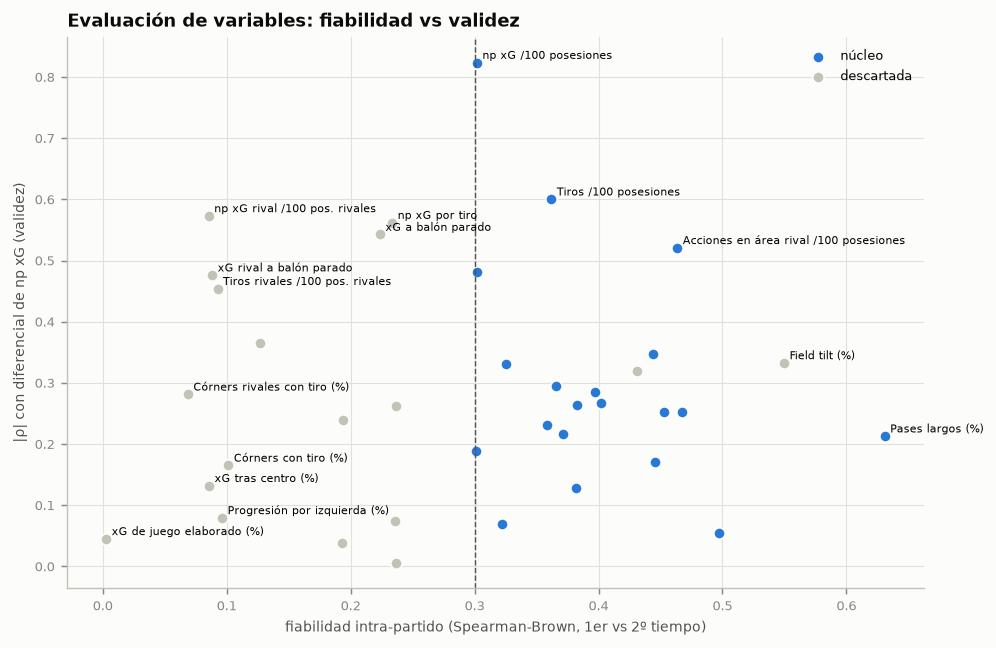
\includegraphics[width=0.82\linewidth]{variable_evaluation.png}
\caption{Fiabilidad intra-partido frente a validez. A la derecha de la línea punteada, variables con fiabilidad
suficiente; en azul, las variables núcleo.}
\label{fig:varEval}
\end{figure}

\begin{aviso}[Hallazgo: el balón parado y el xG concedido son demasiado ruidosos por partido]
Las métricas de balón parado y de ocasiones concedidas tienen una fiabilidad intra-partido cercana a cero: dependen de
pocos eventos raros. Sirven para \emph{describir} un partido en la ficha, pero no como criterio estable ni como variable
explicativa. En cambio, las métricas de volumen y altura (pases largos, field tilt, PPDA, altura de pase, saques de meta
cortos) sí reflejan un rasgo del partido que se sostiene entre los dos tiempos.
\end{aviso}

\subsection{Evolución en el tiempo}
\begin{figure}[H]
\centering
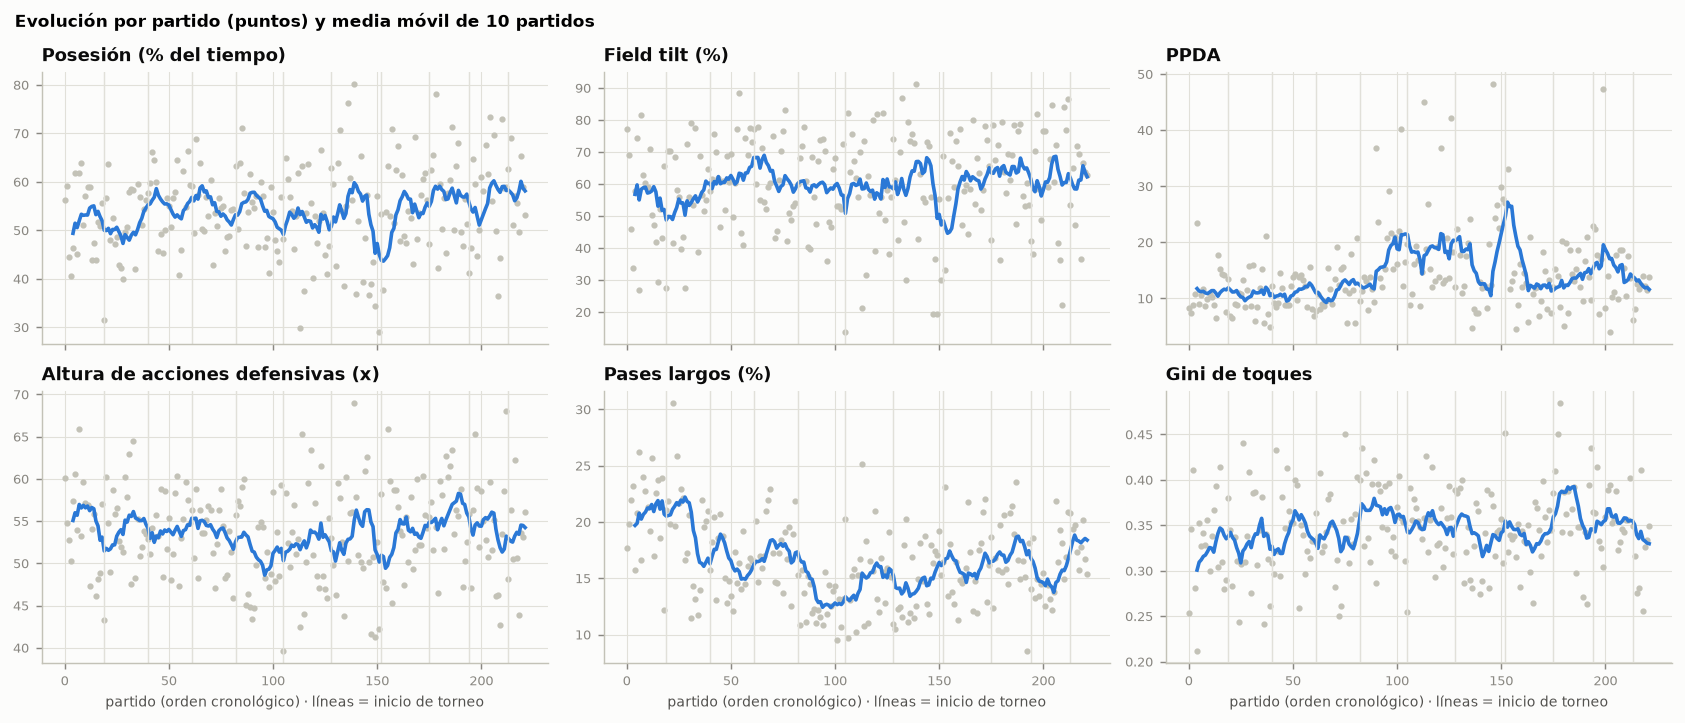
\includegraphics[width=\linewidth]{evolution.png}
\caption{Evolución por partido (puntos) y media móvil de 10 partidos de seis variables núcleo. Las líneas verticales
marcan el inicio de cada torneo.}
\label{fig:evolution}
\end{figure}

% =====================================================================
\section{Reglas contra \emph{data leakage}}\label{sec:leakage}
% =====================================================================
El \emph{data leakage} ocurre cuando el modelo usa información que no estaría disponible en el momento de la
predicción. Produce métricas optimistas que no se sostienen en la práctica. Cada riesgo tiene una regla y una prueba
automática (\texttt{pytest}, 9 pruebas en verde):

\begin{center}
\small
\begin{tabular}{p{4.6cm} p{5.6cm} p{4.4cm}}
\toprule
\textbf{Riesgo} & \textbf{Regla} & \textbf{Verificación} \\
\midrule
Fuerza del rival calculada con partidos futuros & Puntos por partido en los 17 partidos de liga \emph{previos} a la fecha & \texttt{test\_rival\_strength\_uses\_only\_past} \\
Inercia que incluye el propio partido & Media móvil con \texttt{shift(1)} & \texttt{test\_inertia\_is\_lagged} \\
Referencia del jugador que incluye el partido & \texttt{shift(1)} y ventana de 10 & \texttt{test\_player\_reference\_is\_shifted} \\
Escalado, imputación, PCA, clústeres o percentiles ajustados con prueba & Todo dentro de un \texttt{Pipeline}, ajustado solo con entrenamiento & Diseño de \texttt{modeling.py} \\
Objetivo disfrazado en T3 & $x$ = solo métricas de proceso (sin xG, tiros ni OBV) & \texttt{test\_t3\_has\_no\_outcome\_features} \\
Posesiones de un mismo partido en entrenamiento y prueba & Partición \emph{por partido} & \texttt{test\_temporal\_split\_\dots} \\
T4 usa lo que ocurre durante la posesión & $x$ = solo información disponible al inicio & Diseño de \texttt{POSS\_NUM}/\texttt{POSS\_CAT} \\
\bottomrule
\end{tabular}
\end{center}

% =====================================================================
\section{Partición y validación}\label{sec:particion}
% =====================================================================
Los partidos no son independientes ni idénticamente distribuidos: el estilo evoluciona. Una partición aleatoria
filtraría el futuro al entrenamiento. Por eso se usa una partición \textbf{temporal oficial por partido}
(Tabla~\ref{tab:split}):
\begin{itemize}
  \item \textbf{Entrenamiento}: la ventana de datos oficial del hackathon, Apertura 2021 -- Clausura 2025 (\nTrain{}
        partidos del América y toda la liga en el mismo periodo).
  \item \textbf{Validación}: Apertura 2025 (\nVal{} partidos), para elegir la familia de modelo.
  \item \textbf{Prueba}: 2026 (\nTest{} partidos, desde el \testDesde), que se usa \textbf{una sola vez}. Incluye un
        escenario real y exigente: la llegada de un \textbf{técnico nuevo} (Almada) que ningún modelo vio en el América.
\end{itemize}

\begin{table}[H]
\centering
\footnotesize
\caption{Partición temporal por partido.}
\label{tab:split}
\resizebox{\ifdim\width>\linewidth\linewidth\else\width\fi}{!}{%
\begin{tabular}{lrll p{7cm}}
\toprule
\textbf{split} & \textbf{partidos} & \textbf{desde} & \textbf{hasta} & \textbf{torneos} \\
\midrule
train & 175 & 2021-07-23 & 2025-05-26 & Apertura 2021, Clausura 2022, Apertura 2022, Clausura 2023, Apertura 2023, Clausura 2024, Apertura 2024, Clausura 2025 \\
val & 19 & 2025-07-12 & 2025-11-29 & Apertura 2025 \\
test & 28 & 2026-01-10 & 2026-09-28 & Clausura 2026, Apertura 2026 \\
\bottomrule
\end{tabular}}
\end{table}

\begin{itemize}
  \item \textbf{Hiperparámetros}: validación cruzada de \emph{ventana creciente} (\texttt{TimeSeriesSplit}, 4 pliegues)
        \emph{dentro del entrenamiento}, con búsqueda en malla. Siempre se entrena con el pasado y se valida con el
        futuro inmediato. La familia de modelo (Ridge, LASSO, árbol o KNN) se elige con la validación.
  \item \textbf{Preprocesamiento}: estandarización e imputación con estadísticas de entrenamiento, y one-hot con
        \texttt{drop="first"} para evitar la trampa de las variables ficticias. Todo va dentro del \texttt{Pipeline}.
  \item \textbf{Baselines}: en regresión, la media histórica de entrenamiento y la media móvil de los 5 partidos previos
        (inercia); en clasificación, la clase mayoritaria o la tasa base. Un modelo solo "supera al baseline" si le gana
        al \emph{mejor} de los dos (criterio conservador).
\end{itemize}

% =====================================================================
\section{Tareas, modelos y resultados base}\label{sec:modelos}
% =====================================================================
Para cada tarea se reporta la formulación (Tabla~\ref{tab:tareas}), el desempeño en prueba frente al baseline y, cuando
aplica, el diagnóstico de supuestos. Los parámetros (coeficientes, cortes del árbol, centroides) se aprenden de los
datos. Los hiperparámetros (penalización $\alpha$ o $C$, profundidad, número de vecinos, $k$) se eligen por validación
cruzada.

\subsection{T1 · Ajuste al contexto previo (5.2)}
\textbf{$y$}: cada una de 12 variables de estilo. \textbf{$x$}: lo que se sabe \emph{antes} del partido (localía, fuerza
del rival, fase, días de descanso y orden cronológico) más la inercia (media de los 5 partidos previos). \textbf{Modelos}:
Ridge y LASSO (regresión lineal con penalización L2 y L1, que reducen la varianza), árbol de decisión (no lineal e
interpretable) y KNN.

\begin{table}[H]
\centering
\small
\caption{T1 -- MAE en la prueba temporal: mejor modelo (elegido por validación cruzada) frente a los dos baselines.}
\label{tab:t1}
\resizebox{\ifdim\width>\linewidth\linewidth\else\width\fi}{!}{%
\begin{tabular}{lrrrrrr}
\toprule
\textbf{variable} & \textbf{modelo} & \textbf{media hist.} & \textbf{media móvil 5} & \textbf{modelo} & \textbf{$R^2$} & \textbf{mejora (\%)} \\
\midrule
Posesión (\% del tiempo) & Árbol & 8.48 & 9.15 & 7.70 & 0.07 & 9.20 \\
Field tilt (\%) & KNN & 14.24 & 15.84 & 13.32 & -0.03 & 6.50 \\
PPDA & Ridge & 4.92 & 5.76 & 5.25 & 0.03 & -6.72 \\
Altura de acciones defensivas (x) & Árbol & 4.67 & 5.73 & 4.96 & -0.12 & -6.24 \\
Acciones defensivas en campo rival (\%) & Árbol & 7.11 & 8.60 & 7.24 & -0.09 & -1.87 \\
Altura media de pase (x) & Ridge & 4.34 & 4.91 & 4.38 & -0.07 & -0.87 \\
Pases progresivos /100 pases & KNN & 1.36 & 1.40 & 1.42 & -0.11 & -4.27 \\
Pases largos (\%) & LASSO & 2.37 & 2.00 & 2.14 & -0.07 & -6.78 \\
Saques de meta cortos (\%) & LASSO & 26.17 & 24.04 & 23.58 & -0.27 & 1.90 \\
Posesiones en transición (\%) & Ridge & 3.71 & 4.03 & 4.03 & -0.31 & -8.70 \\
np xG /100 posesiones & Ridge & 0.50 & 0.46 & 0.55 & -0.45 & -18.59 \\
np xG rival /100 pos. rivales & KNN & 0.48 & 0.51 & 0.46 & -0.12 & 3.15 \\
\bottomrule
\end{tabular}}
\end{table}

\begin{historia}[Lectura de T1: identidad estable más ruido, con ajustes claros al contexto]
\begin{itemize}
  \item El modelo supera al mejor baseline en \nTunoSupera{} de \nTuno{} variables, con mejoras modestas (hasta
        \tunoMejoraMax\,\%) y un $R^2$ de prueba cercano a 0. La \emph{media histórica} suele ganarle a la inercia: el
        estilo por partido se comporta como una identidad estable más ruido, no como una tendencia que se arrastra.
  \item Aun así, el contexto mueve el estilo de forma sistemática (Figura~\ref{fig:t1}). Por cada punto por partido
        adicional de fuerza del rival, la posesión baja \rivalPos{} puntos, el field tilt \rivalTilt{} y los pases largos
        suben \rivalLong. De local, el field tilt sube \localTilt{} puntos y las acciones defensivas en campo rival
        \localPress.
\end{itemize}
\end{historia}

\begin{figure}[H]
\centering
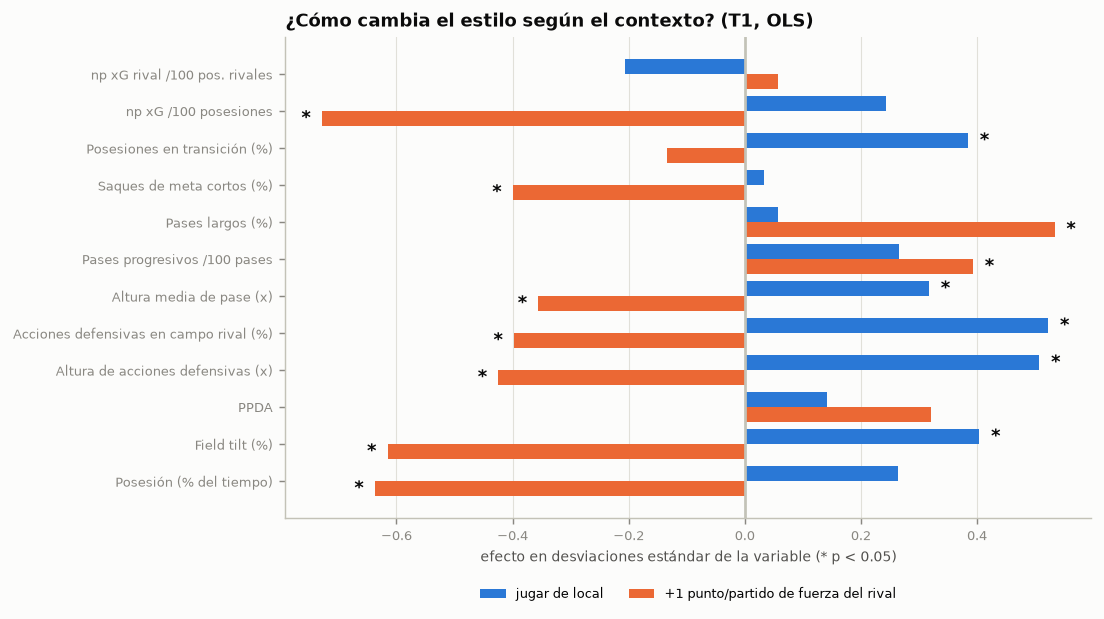
\includegraphics[width=0.92\linewidth]{t1_context_effects.png}
\caption{Efecto de la localía y de la fuerza del rival sobre cada variable de estilo (OLS, en desviaciones estándar de
la variable; $*$: $p<0.05$).}
\label{fig:t1}
\end{figure}

\paragraph{Supuestos del modelo lineal.} Para interpretar coeficientes se ajusta un OLS con las mismas $x$ y se
diagnostican los supuestos (Tabla~\ref{tab:t1Assump}):
\begin{itemize}
  \item \textbf{Independencia}: el Durbin-Watson ronda 2, porque la inercia absorbe la dependencia temporal.
  \item \textbf{Homocedasticidad}: Breusch-Pagan no la rechaza en ninguna variable.
  \item \textbf{Normalidad}: Jarque-Bera la rechaza en las variables con colas pesadas (PPDA, xG propio y xG rival) y,
        marginalmente, en field tilt y saques de meta cortos. Eso no afecta la
        predicción, pero sí los intervalos, por lo que se interpreta el tamaño del efecto antes que el valor $p$.
  \item \textbf{Multicolinealidad}: el VIF máximo es menor que 2, así que no hay multicolinealidad entre las $x$.
\end{itemize}

\begin{table}[H]
\centering
\small
\caption{T1 -- Diagnóstico de supuestos del modelo lineal (OLS en entrenamiento + validación).}
\label{tab:t1Assump}
\resizebox{\ifdim\width>\linewidth\linewidth\else\width\fi}{!}{%
\begin{tabular}{lrrrrr}
\toprule
\textbf{variable} & \textbf{$R^2$ train} & \textbf{Durbin-Watson} & \textbf{BP (p)} & \textbf{JB (p)} & \textbf{VIF máx} \\
\midrule
Posesión (\% del tiempo) & 0.099 & 2.030 & 0.426 & 0.560 & 1.322 \\
Field tilt (\%) & 0.122 & 1.926 & 0.294 & 0.046 & 1.257 \\
PPDA & 0.188 & 1.908 & 0.218 & 0.000 & 1.409 \\
Altura de acciones defensivas (x) & 0.118 & 2.059 & 0.202 & 0.612 & 1.275 \\
Acciones defensivas en campo rival (\%) & 0.118 & 2.146 & 0.245 & 0.539 & 1.274 \\
Altura media de pase (x) & 0.054 & 1.748 & 0.725 & 0.454 & 1.255 \\
Pases progresivos /100 pases & 0.057 & 2.068 & 0.444 & 0.888 & 1.246 \\
Pases largos (\%) & 0.304 & 1.813 & 0.822 & 0.082 & 1.602 \\
Saques de meta cortos (\%) & 0.129 & 1.909 & 0.535 & 0.044 & 1.254 \\
Posesiones en transición (\%) & 0.078 & 2.138 & 0.333 & 0.089 & 1.255 \\
np xG /100 posesiones & 0.143 & 2.063 & 0.443 & 0.000 & 1.247 \\
np xG rival /100 pos. rivales & 0.021 & 2.277 & 0.923 & 0.000 & 1.255 \\
\bottomrule
\end{tabular}}
\end{table}

\subsection{T2 · Ajuste intra-partido: marcador y momento (5.2)}
\textbf{$y$}: el estilo en cada tramo de 15' con estado del marcador (\nSegmentos{} segmentos). \textbf{$x$}: estado del
marcador, tramo, localía, fase y fuerza del rival. \textbf{Modelos}: Ridge y árbol.

\begin{table}[H]
\centering
\small
\caption{T2 -- MAE en prueba por tramo de 15' y estado del marcador.}
\label{tab:t2}
\resizebox{\ifdim\width>\linewidth\linewidth\else\width\fi}{!}{%
\begin{tabular}{lrrrr}
\toprule
\textbf{variable} & \textbf{baseline} & \textbf{Ridge} & \textbf{Árbol} & \textbf{$R^2$ Ridge} \\
\midrule
Posesión (\% del tiempo) & 15.24 & 14.37 & 14.73 & 0.07 \\
Field tilt (\%) & 23.23 & 21.04 & 21.76 & 0.13 \\
Altura media de pase (x) & 8.46 & 7.90 & 8.28 & 0.10 \\
Altura de acciones defensivas (x) & 9.62 & 9.19 & 9.20 & 0.07 \\
Acciones defensivas en campo rival (\%) & 13.89 & 13.46 & 13.46 & 0.06 \\
Pases largos (\%) & 5.70 & 5.68 & 5.57 & -0.01 \\
\bottomrule
\end{tabular}}
\end{table}

\begin{figure}[H]
\centering
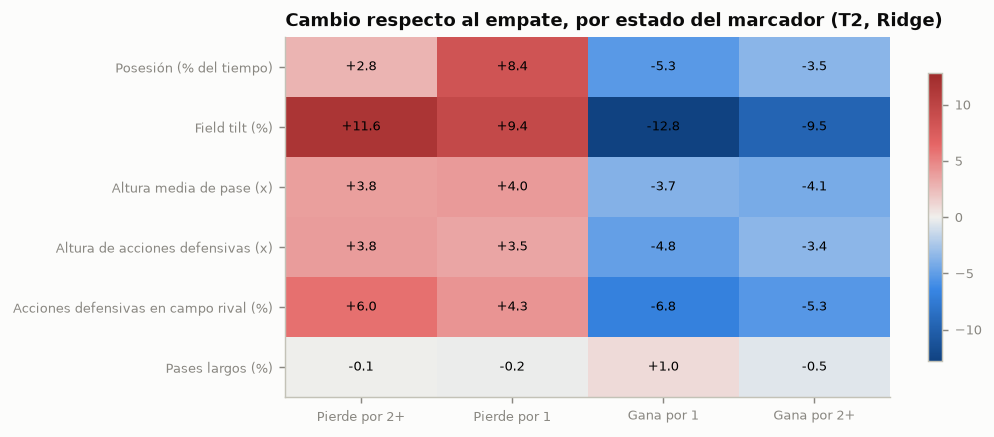
\includegraphics[width=0.78\linewidth]{t2_game_state.png}
\caption{Coeficientes de Ridge del estado del marcador: diferencia respecto al empate, en unidades de cada variable.}
\label{fig:t2}
\end{figure}

\begin{historia}[Lectura de T2: el marcador cambia el plan]
Ridge supera al baseline en las seis variables. El patrón es claro y simétrico: perdiendo por un gol, el field tilt
sube \tiltPierde{} puntos y la posesión \posPierde; ganando por uno, bajan \tiltGana{} y \posGana. El equipo adelanta la
presión y el bloque cuando necesita el gol y se repliega cuando lo protege. Parte del efecto es universal en el fútbol
(el rival también ajusta), por lo que la comparación útil será entre periodos y entrenadores con la misma medida.
\end{historia}

\subsection{T3 · Principios que generan dominio (5.1, 5.5) y T3b · resultado}
\textbf{$y$}: OBV neto y diferencial de np xG. \textbf{$x$}: 24 métricas de \emph{proceso}; se excluyen xG, tiros, OBV y
sus derivados para evitar un objetivo disfrazado. \textbf{Modelos}: LASSO, cuya penalización L1 selecciona variables,
con estabilidad medida en 100 remuestreos bootstrap; árbol y KNN.

\begin{table}[H]
\centering
\small
\caption{T3 -- MAE en prueba de los modelos de dominio con métricas de proceso.}
\label{tab:t3}
\resizebox{\ifdim\width>\linewidth\linewidth\else\width\fi}{!}{%
\begin{tabular}{lrrrrrrr}
\toprule
\textbf{objetivo} & \textbf{MAE baseline} & \textbf{MAE LASSO} & \textbf{MAE Árbol} & \textbf{MAE KNN} & \textbf{R2 LASSO} & \textbf{alpha} & \textbf{variables elegidas} \\
\midrule
OBV neto & 1.408 & 1.408 & 1.507 & 1.483 & -0.001 & 0.500 & 0 \\
Diferencial np xG & 0.655 & 0.548 & 0.556 & 0.581 & 0.130 & 0.100 & 6 \\
\bottomrule
\end{tabular}}
\end{table}
\begin{table}[H]
\centering
\small
\caption{T3 -- Variables elegidas por LASSO para el diferencial de np xG: coeficiente (x estandarizadas) y estabilidad (\% de 100 remuestreos bootstrap en que se elige).}
\label{tab:t3Lasso}
\resizebox{\ifdim\width>\linewidth\linewidth\else\width\fi}{!}{%
\begin{tabular}{lrr}
\toprule
\textbf{etiqueta} & \textbf{coef} & \textbf{estabilidad} \\
\midrule
Acciones en área rival /100 posesiones & 0.355 & 1.000 \\
Gini de toques & 0.100 & 0.930 \\
Precisión bajo presión en tercio propio (\%) & 0.072 & 0.860 \\
Pases progresivos /100 pases & 0.031 & 0.740 \\
Posesiones rivales que llegan a último tercio (\%) & -0.075 & 0.720 \\
Pases por construcción & 0.004 & 0.370 \\
Altura de acciones defensivas (x) & 0.000 & 0.310 \\
\bottomrule
\end{tabular}}
\end{table}

\begin{itemize}
  \item \textbf{Diferencial de np xG}: LASSO mejora al baseline ($R^2=\tresRdos$) con \tresNvar{} principios de proceso
        estables. En orden: más acciones en el área rival, juego más repartido (Gini de toques), precisión bajo presión
        en la salida y progresión por pase, y menos llegadas del rival al último tercio.
  \item \textbf{OBV neto}: la validación cruzada elige el modelo nulo, porque ninguna métrica de proceso lo explica mejor
        que la media. El OBV neto de un partido es muy ruidoso, y el diferencial de xG es mejor objetivo de "dominio".
  \item \textbf{T3b} (resultado G/E/P, Tabla~\ref{tab:t3b}): los modelos mejoran el F1 macro frente a predecir siempre
        victoria, pero el resultado depende de la conversión, que es mayormente azar. Por eso la ficha explica el
        resultado con la simulación del xG (Sección~\ref{sec:implementacion}) y no con un clasificador.
\end{itemize}

\begin{table}[H]
\centering
\small
\caption{T3b -- Resultado del partido (G/E/P) en prueba.}
\label{tab:t3b}
\resizebox{\ifdim\width>\linewidth\linewidth\else\width\fi}{!}{%
\begin{tabular}{lrr}
\toprule
\textbf{modelo} & \textbf{exactitud} & \textbf{F1 macro} \\
\midrule
Baseline: clase mayoritaria (W) & 0.464 & 0.211 \\
Logística softmax & 0.357 & 0.310 \\
Árbol & 0.357 & 0.376 \\
\bottomrule
\end{tabular}}
\end{table}

\subsection{T4 · Posesión $\rightarrow$ ocasión (5.1) y T5 · balón parado (5.4)}
Ambas son clasificaciones binarias desbalanceadas: solo el \cuatroPrev\,\% de las posesiones del equipo termina en
tiro. Se usa \texttt{class\_weight="balanced"}, que mejora la \emph{discriminación} (ROC-AUC de \cuatroAUC{} en T4) pero
\emph{descalibra} las probabilidades; por eso el Brier empeora frente a la tasa base. Para comparar posesiones o
jugadas basta con discriminar bien; para usar la probabilidad como tal habría que recalibrarla (por ejemplo, con
Platt o isotónica). Las \emph{model cards} lo registran en el campo \texttt{calibrated}.

\begin{table}[H]
\centering
\small
\caption{T4 -- ¿La posesión termina en tiro? Métricas en prueba.}
\label{tab:t4}
\resizebox{\ifdim\width>\linewidth\linewidth\else\width\fi}{!}{%
\begin{tabular}{lrrrr}
\toprule
\textbf{modelo} & \textbf{ROC-AUC} & \textbf{prevalencia} & \textbf{F1} & \textbf{Brier} \\
\midrule
Baseline: tasa base & 0.500 & 0.122 & -- & 0.126 \\
Logística & 0.719 & -- & 0.364 & 0.217 \\
Árbol & 0.689 & -- & 0.375 & 0.212 \\
KNN & 0.711 & -- & 0.076 & 0.113 \\
\bottomrule
\end{tabular}}
\end{table}
\begin{table}[H]
\centering
\small
\caption{T4 -- Coeficientes de la regresión logística (log-odds, x estandarizadas): los 6 más negativos y los 6 más positivos.}
\label{tab:t4Coefs}
\resizebox{\ifdim\width>\linewidth\linewidth\else\width\fi}{!}{%
\begin{tabular}{lr}
\toprule
\textbf{variable (one-hot)} & \textbf{coef (log-odds, x estandarizadas)} \\
\midrule
play\_pattern\_From Kick Off & -1.219 \\
play\_pattern\_From Throw In & -0.662 \\
play\_pattern\_From Keeper & -0.394 \\
play\_pattern\_From Goal Kick & -0.324 \\
play\_pattern\_Regular Play & -0.279 \\
start\_y\_abs & -0.219 \\
minute\_bin\_45-60 & 0.253 \\
minute\_bin\_60-75 & 0.310 \\
minute\_bin\_90+ & 0.340 \\
minute\_bin\_75-90 & 0.347 \\
start\_type\_c\_Otro & 0.475 \\
start\_x & 0.685 \\
\bottomrule
\end{tabular}}
\end{table}
\begin{table}[H]
\centering
\small
\caption{T5 -- ¿El balón parado termina en tiro? Métricas en prueba.}
\label{tab:t5}
\resizebox{\ifdim\width>\linewidth\linewidth\else\width\fi}{!}{%
\begin{tabular}{lrrrr}
\toprule
\textbf{conjunto · modelo} & \textbf{ROC-AUC} & \textbf{prevalencia} & \textbf{F1} & \textbf{Brier} \\
\midrule
A favor · Baseline: tasa base & 0.500 & 0.181 & -- & 0.177 \\
A favor · Logística & 0.683 & -- & 0.478 & 0.214 \\
A favor · Árbol & 0.670 & -- & 0.457 & 0.211 \\
En contra · Baseline: tasa base & 0.500 & 0.165 & -- & 0.135 \\
En contra · Logística & 0.710 & -- & 0.414 & 0.205 \\
En contra · Árbol & 0.707 & -- & 0.400 & 0.202 \\
\bottomrule
\end{tabular}}
\end{table}
\begin{table}[H]
\centering
\small
\caption{T5 -- Balón parado a favor: \% que termina en tiro por tipo y zona de destino (grupos con $\geq$ 20 jugadas).}
\label{tab:t5Rates}
\resizebox{\ifdim\width>\linewidth\linewidth\else\width\fi}{!}{%
\begin{tabular}{lrrr}
\toprule
\textbf{tipo · zona} & \textbf{jugadas} & \textbf{\% tiro} & \textbf{xG} \\
\midrule
Córner · Zona de penal & 536 & 0.45 & 22.08 \\
Córner · Área (costados) & 78 & 0.36 & 1.79 \\
Tiro libre · Área chica & 64 & 0.31 & 3.54 \\
Saque de banda · Zona de penal & 27 & 0.30 & 0.47 \\
Tiro libre · Zona de penal & 291 & 0.30 & 8.20 \\
Córner · Área chica & 224 & 0.29 & 8.86 \\
Córner · Corto & 428 & 0.26 & 12.15 \\
Tiro libre · Corto & 960 & 0.24 & 16.66 \\
Córner · Fuera del área & 362 & 0.19 & 9.26 \\
Saque de banda · Área (costados) & 164 & 0.14 & 1.68 \\
Tiro libre · Área (costados) & 125 & 0.14 & 1.61 \\
Saque de banda · Fuera del área & 768 & 0.13 & 9.95 \\
Saque de banda · Corto & 709 & 0.10 & 6.99 \\
Tiro libre · Fuera del área & 1,899 & 0.10 & 25.62 \\
\bottomrule
\end{tabular}}
\end{table}

\subsection{T6 · Impacto de las sustituciones (5.3)}
\textbf{$y$}: el cambio en OBV neto, field tilt y np xG entre los 15' anteriores y los 15' posteriores a cada intervención
(\nCambios{} intervenciones; los cambios hechos en un mismo minuto cuentan como una). \textbf{$x$}: minuto, marcador,
número de cambios, líneas que salen, localía y rival.

\begin{table}[H]
\centering
\small
\caption{T6 -- Impacto de las sustituciones: MAE en prueba frente a dos baselines.}
\label{tab:t6}
\resizebox{\ifdim\width>\linewidth\linewidth\else\width\fi}{!}{%
\begin{tabular}{lrrrrr}
\toprule
\textbf{objetivo} & \textbf{Baseline: sin cambio ($\Delta$=0)} & \textbf{Baseline: $\Delta$ medio} & \textbf{Ridge} & \textbf{Árbol} & \textbf{R2 Ridge} \\
\midrule
\$\textbackslash\{\}Delta\$ OBV neto & 0.711 & 0.712 & 0.704 & 0.706 & 0.041 \\
\$\textbackslash\{\}Delta\$ field tilt & 22.812 & 22.810 & 22.967 & 23.214 & -0.024 \\
\$\textbackslash\{\}Delta\$ np xG & 0.317 & 0.317 & 0.322 & 0.332 & -0.017 \\
\bottomrule
\end{tabular}}
\end{table}

Ningún modelo mejora de forma relevante a los baselines ("el cambio no altera nada" o el cambio medio): a lo sumo 1\,\%
en $\Delta$ OBV neto y peor en las otras dos. Con la información disponible, el efecto de un cambio es
\textbf{impredecible} intervención por intervención. Es un resultado honesto: la ficha muestra el antes y el después de
cada cambio (Figura~\ref{fig:fichaTimeline}), pero no promete su efecto.

\subsection{T7 · Distribución del juego según el contexto (5.3 + 5.2)}
\begin{table}[H]
\centering
\small
\caption{T7 -- Distribución del juego según el contexto: MAE en prueba.}
\label{tab:t7}
\resizebox{\ifdim\width>\linewidth\linewidth\else\width\fi}{!}{%
\begin{tabular}{lrrrr}
\toprule
\textbf{variable} & \textbf{modelo} & \textbf{MAE modelo} & \textbf{media móvil 5} & \textbf{media hist.} \\
\midrule
Gini de toques & Ridge & 0.036 & 0.039 & 0.033 \\
Gini de progresión & LASSO & 0.064 & 0.063 & 0.064 \\
OBV de los 3 mejores (\%) & Árbol & 7.803 & 8.417 & 8.017 \\
OBV p90 vs referencia (media) & LASSO & 0.101 & 0.102 & 0.101 \\
\bottomrule
\end{tabular}}
\end{table}
La concentración del juego y la potenciación de los jugadores apenas dependen del contexto previo: solo la dependencia
de los tres mejores y la potenciación mejoran ligeramente a la media histórica. El reparto del juego es un rasgo del partido y no algo
que se anticipe desde el calendario.

\subsection{U1 / U2 · Ejes de estilo y tipos de partido}
\textbf{U1}: PCA sobre las 12 variables de estilo, ajustado solo con entrenamiento; se retienen las \nPC{} componentes
necesarias para superar el 70\,\% de la varianza. La primera (\pcUnoVar\,\%) es un eje de \emph{dominio territorial}:
field tilt, altura de acciones defensivas y presión alta. \textbf{U2}: K-means sobre las componentes, con $k$ elegido
por silhouette ($k=2$, silhouette $=\silDos$).

\begin{table}[H]
\centering
\small
\caption{U2 -- Perfil medio de cada tipo de partido (entrenamiento).}
\label{tab:u2}
\resizebox{\ifdim\width>\linewidth\linewidth\else\width\fi}{!}{%
\begin{tabular}{lrr}
\toprule
\textbf{variable (media en train)} & \textbf{Tipo 1} & \textbf{Tipo 2} \\
\midrule
Posesión (\% del tiempo) & 57.98 & 46.07 \\
Field tilt (\%) & 68.83 & 44.34 \\
PPDA & 11.68 & 18.53 \\
Altura de acciones defensivas (x) & 56.27 & 48.89 \\
Acciones defensivas en campo rival (\%) & 45.50 & 35.54 \\
Altura media de pase (x) & 60.92 & 54.59 \\
Pases progresivos /100 pases & 7.10 & 6.73 \\
Pases largos (\%) & 15.79 & 17.66 \\
Saques de meta cortos (\%) & 48.08 & 30.68 \\
Posesiones en transición (\%) & 19.42 & 15.42 \\
np xG /100 posesiones & 1.51 & 1.20 \\
np xG rival /100 pos. rivales & 0.75 & 0.90 \\
\bottomrule
\end{tabular}}
\end{table}

\begin{figure}[H]
\centering
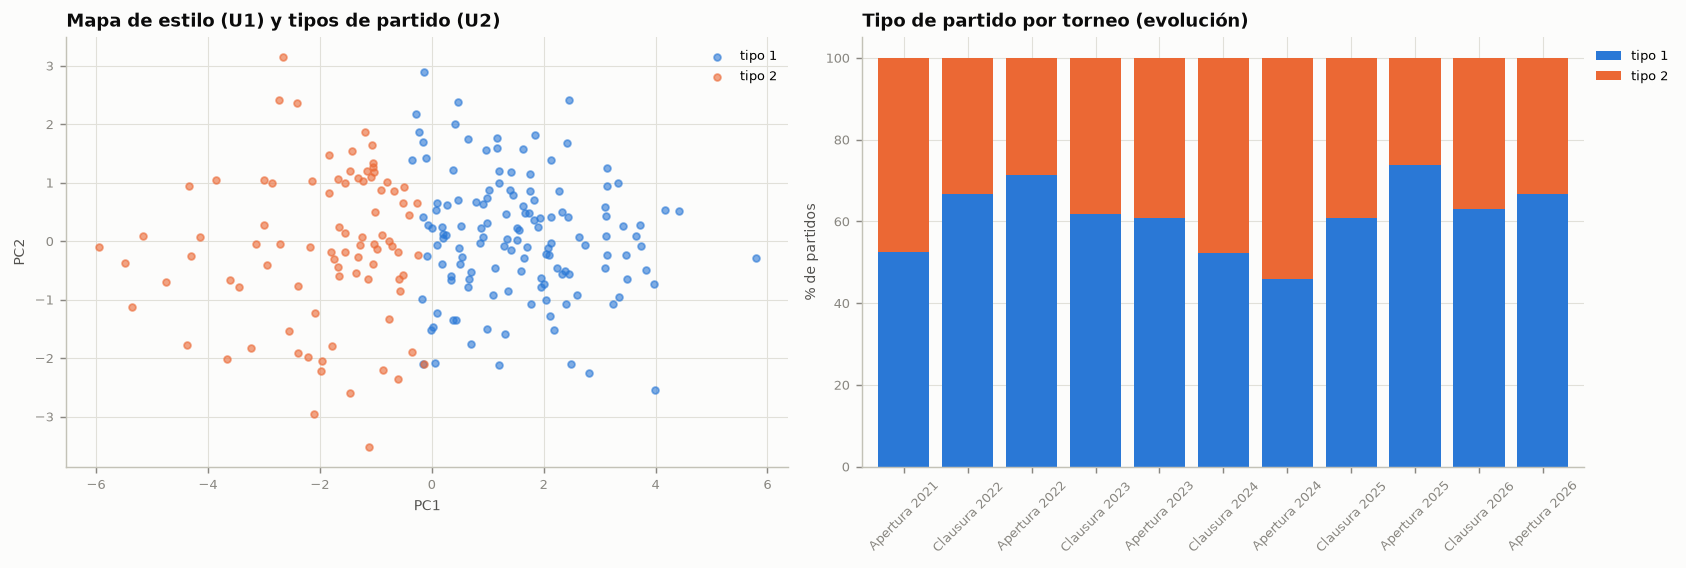
\includegraphics[width=\linewidth]{u1u2_style.png}
\caption{Mapa de estilo (dos primeras componentes) con el tipo de partido, y porcentaje de cada tipo por torneo.}
\label{fig:u1u2}
\end{figure}

\begin{historia}[Dos tipos de partido]
\begin{itemize}
  \item \textbf{Tipo 1, dominante}: posesión \tipoUnoPos\,\%, field tilt \tipoUnoTilt\,\%, PPDA \tipoUnoPPDA.
  \item \textbf{Tipo 2, reactivo}: posesión \tipoDosPos\,\%, field tilt \tipoDosTilt\,\%, PPDA \tipoDosPPDA.
\end{itemize}
El equipo juega partidos del tipo 1 en la mayoría de los torneos, pero la proporción cambia por torneo (Tabla~\ref{tab:u2Torneo}). El
Apertura 2024, campeón, fue el torneo más reactivo; el Apertura 2025, el más dominante. La silhouette moderada indica un
\emph{continuo} de estilo más que grupos separados: los tipos son una simplificación útil para la ficha.
\end{historia}

\begin{table}[H]
\centering
\small
\caption{U2 -- Porcentaje de partidos de cada tipo por torneo.}
\label{tab:u2Torneo}
\resizebox{\ifdim\width>\linewidth\linewidth\else\width\fi}{!}{%
\begin{tabular}{lrr}
\toprule
\textbf{torneo} & \textbf{Tipo 1 (\textbackslash\{\}\%)} & \textbf{Tipo 2 (\textbackslash\{\}\%)} \\
\midrule
Apertura 2021 & 53 & 47 \\
Clausura 2022 & 67 & 33 \\
Apertura 2022 & 71 & 29 \\
Clausura 2023 & 62 & 38 \\
Apertura 2023 & 61 & 39 \\
Clausura 2024 & 52 & 48 \\
Apertura 2024 & 46 & 54 \\
Clausura 2025 & 61 & 39 \\
Apertura 2025 & 74 & 26 \\
Clausura 2026 & 63 & 37 \\
Apertura 2026 & 67 & 33 \\
\bottomrule
\end{tabular}}
\end{table}

\subsection{U3 · Roles de jugador (5.3)}
K-means sobre perfiles por 90' (jugador $\times$ partido con al menos 30 minutos, sin porteros; 14 acciones), ajustado
con entrenamiento. Se identifican \nRoles{} roles (Tabla~\ref{tab:u3}, Figura~\ref{fig:u3}): un rol de
\emph{distribución} (muchos toques y pases, dominado por medios defensivos), uno de \emph{recuperación}
(defensas), uno de \emph{creación} (xA y OBV de pase), uno de \emph{finalización y presión} (delanteros) y uno de
\emph{regate y conducción} (bandas). La silhouette baja ($\silRoles$) indica que los roles se solapan: un mismo jugador
cambia de rol entre partidos, que es justo lo que interesa medir en el encaje rol--uso.

\begin{table}[H]
\centering
\small
\caption{U3 -- Roles de jugador (K-means sobre perfiles p90, ajustado con train).}
\label{tab:u3}
\resizebox{\ifdim\width>\linewidth\linewidth\else\width\fi}{!}{%
\begin{tabular}{lrrr}
\toprule
\textbf{rol} & \textbf{posición dominante} & \textbf{\% posición dominante} & \textbf{jugador-partidos} \\
\midrule
Rol 1: touches + passes & Medio defensivo & 58 & 395 \\
Rol 2: interceptions + ball\_recoveries & Defensa & 67 & 971 \\
Rol 3: xa + obv\_pass & Banda & 37 & 155 \\
Rol 4: np\_xg + pressures & Delantero & 42 & 688 \\
Rol 5: dribbles + obv\_dribble\_carry & Banda & 53 & 331 \\
\bottomrule
\end{tabular}}
\end{table}

\begin{figure}[H]
\centering
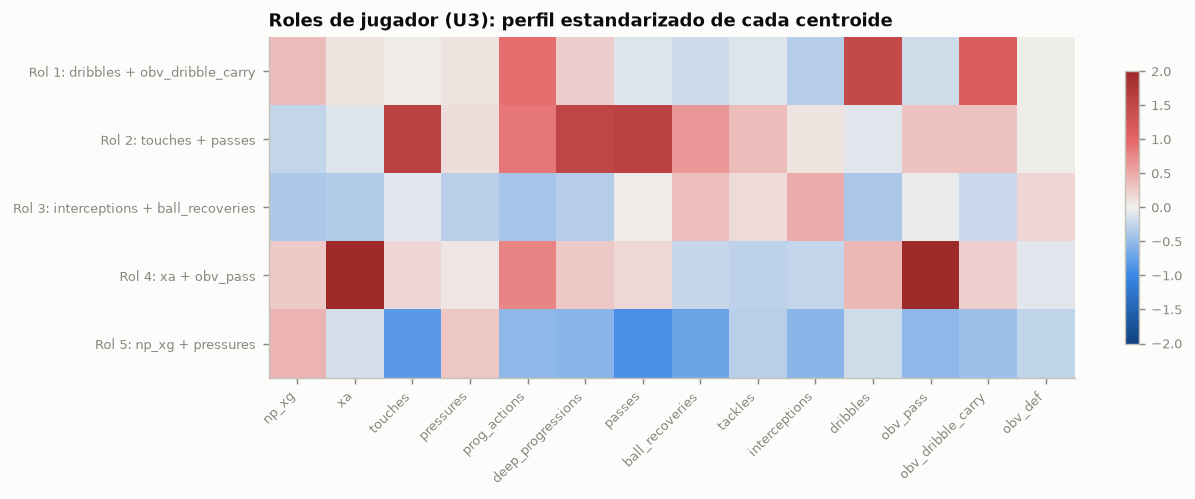
\includegraphics[width=\linewidth]{u3_roles.png}
\caption{Perfil estandarizado de cada rol de jugador (centroides de K-means).}
\label{fig:u3}
\end{figure}

% =====================================================================
\section{Evaluación en la prueba temporal}\label{sec:evaluacion}
% =====================================================================
De \nSupervisados{} modelos supervisados, \nSupera{} superan al mejor baseline en la prueba temporal (Apéndice~\ref{app:cards}).
La Tabla~\ref{tab:overfit} compara el error de los modelos de T1 en entrenamiento, validación y prueba:
\begin{itemize}
  \item Razones prueba/entrenamiento cercanas a 1 indican que el modelo no memorizó.
  \item Razones de 1.1 a 1.35 son esperables: la prueba de 2026 incluye un cambio de técnico. Las más altas (xG rival y
        pases progresivos) coinciden con variables donde el modelo no supera al baseline, y ahí la ficha usa el baseline.
\end{itemize}

\begin{table}[H]
\centering
\small
\caption{Diagnóstico de sobreajuste (T1): MAE del modelo elegido en cada conjunto.}
\label{tab:overfit}
\resizebox{\ifdim\width>\linewidth\linewidth\else\width\fi}{!}{%
\begin{tabular}{lrrrr}
\toprule
\textbf{variable} & \textbf{train} & \textbf{val} & \textbf{test} & \textbf{test / train} \\
\midrule
Acciones defensivas en campo rival (\%) & 5.95 & 5.88 & 7.24 & 1.22 \\
Altura de acciones defensivas (x) & 4.11 & 3.92 & 4.96 & 1.21 \\
Altura media de pase (x) & 3.56 & 4.89 & 4.38 & 1.23 \\
Field tilt (\%) & 11.80 & 9.88 & 13.32 & 1.13 \\
PPDA & 4.64 & 3.66 & 5.25 & 1.13 \\
Pases largos (\%) & 2.82 & 2.83 & 2.14 & 0.76 \\
Pases progresivos /100 pases & 1.10 & 1.21 & 1.42 & 1.29 \\
Posesiones en transición (\%) & 3.79 & 4.81 & 4.03 & 1.07 \\
Posesión (\% del tiempo) & 6.75 & 6.82 & 7.70 & 1.14 \\
Saques de meta cortos (\%) & 19.87 & 23.28 & 23.58 & 1.19 \\
np xG /100 posesiones & 0.57 & 0.42 & 0.55 & 0.95 \\
np xG rival /100 pos. rivales & 0.34 & 0.27 & 0.46 & 1.35 \\
\bottomrule
\end{tabular}}
\end{table}

% =====================================================================
\section{ADN del entrenador: el estilo de cualquier técnico frente a la liga}\label{sec:adn}
% =====================================================================
Predecir un partido es difícil: el estilo por partido es una identidad estable más ruido (T1). Lo que sí es estable,
y lo que pide el reto (\emph{``entender los estilos de juego de entrenadores y las características que los
definen''}), es el \textbf{perfil promedio de un técnico frente a la liga}. Con las estadísticas de equipo de los
1,789 partidos de la Liga MX se construye el \textbf{ADN del entrenador} para los \nTecnicos{} técnicos de la liga
(Notebook 04).

\begin{itemize}
  \item \textbf{8 rasgos de juego} (Tabla~\ref{tab:coachAxes}). Cada rasgo es el promedio de 2 a 4 métricas
        estandarizadas con la liga, orientadas para que ``más'' signifique ``más de ese rasgo''.
  \item \textbf{Ajuste por contexto}: a cada rasgo se le quita el efecto del rival (efecto fijo) y de la localía,
        estimados con la ventana oficial. Así se mide el estilo \emph{del técnico} y no el del calendario.
  \item \textbf{Percentil de liga}: cada rasgo del técnico se ubica entre los técnicos-club con 15 partidos o más en la
        ventana oficial. El 50 corresponde al técnico típico de la Liga MX.
\end{itemize}

\begin{table}[H]
\centering
\footnotesize
\caption{Los 8 rasgos del ADN del entrenador y sus métricas de StatsBomb.}
\label{tab:coachAxes}
\resizebox{\ifdim\width>\linewidth\linewidth\else\width\fi}{!}{%
\begin{tabular}{l p{5.2cm} p{6.4cm}}
\toprule
\textbf{rasgo} & \textbf{métricas (-- = invertida)} & \textbf{qué significa} \\
\midrule
Control del balón & possession, pass\_completion, time\_in\_control & Cuánto tiempo tiene el balón y qué tan seguro lo circula. \\
Verticalidad & directness, pace\_towards\_goal, avg\_team\_possession\_directness & Qué tan rápido y directo va hacia la portería rival en lugar de elaborar. \\
Llegada al área & deep\_progressions, deep\_completions, passes\_inside\_box & Cuántas veces pisa el último tercio y el área rival con el balón. \\
Presión alta & --ppda, fhalf\_pressures\_ratio, defensive\_distance, aggression & Qué tan arriba y qué tan intenso intenta recuperar (menos pases permite al rival). \\
Reacción tras pérdida & counterpressures, counterpressure\_regains & Cuánto presiona justo después de perder el balón y cuánto recupera así. \\
Peligro generado & np\_xg, np\_xg\_per\_shot, obv & Calidad y cantidad de las ocasiones que crea. \\
Solidez defensiva & --np\_xg\_conceded, --deep\_progressions\_conceded, --obv\_conceded & Qué tan poco peligro y qué tan pocas llegadas concede. \\
Balón parado & sp\_xg, xg\_per\_sp, --sp\_xg\_conceded & Peligro a favor en jugadas a balón parado, menos el que concede. \\
\bottomrule
\end{tabular}}
\end{table}

\begin{figure}[H]
\centering
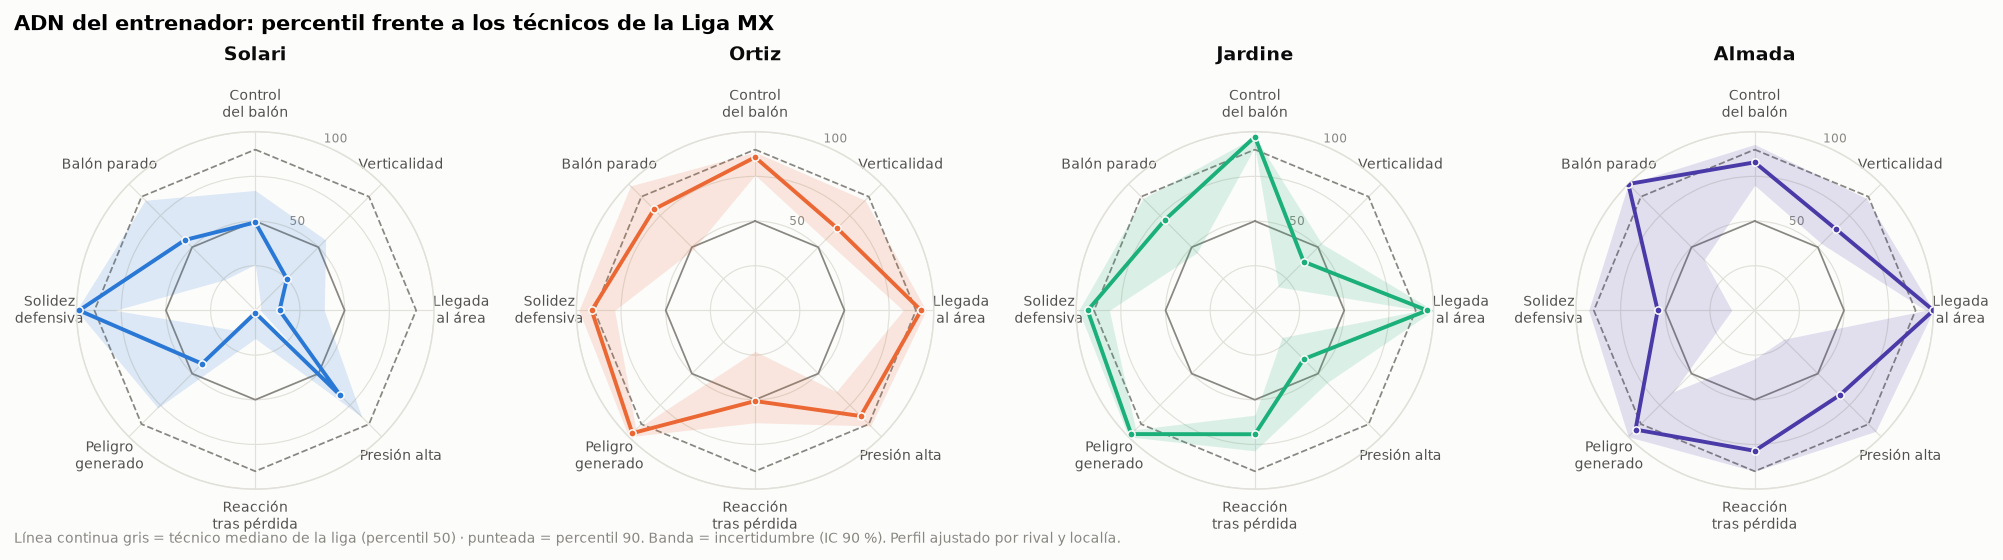
\includegraphics[width=\linewidth]{adn_america.png}
\caption{ADN de los técnicos del América frente a la Liga MX (percentiles; banda = IC 90\,\%). Solari, Ortiz y Jardine
con la ventana oficial; Almada con sus 9 partidos de 2026 (prueba).}
\label{fig:adn}
\end{figure}

\begin{table}[H]
\centering
\footnotesize
\caption{ADN de los técnicos del América: percentil de cada rasgo frente a los técnicos de la Liga MX (ajustado por rival y localía). Almada, con sus partidos de 2026 (prueba).}
\label{tab:coachPct}
\resizebox{\ifdim\width>\linewidth\linewidth\else\width\fi}{!}{%
\begin{tabular}{lrrrrrrrrr}
\toprule
\textbf{técnico} & \textbf{Control del balón} & \textbf{Verticalidad} & \textbf{Llegada al área} & \textbf{Presión alta} & \textbf{Reacción tras pérdida} & \textbf{Peligro generado} & \textbf{Solidez defensiva} & \textbf{Balón parado} & \textbf{partidos} \\
\midrule
Solari & 49 & 25 & 14 & 67 & 1 & 42 & 99 & 56 & 27 \\
Ortiz & 86 & 65 & 93 & 84 & 51 & 97 & 91 & 80 & 55 \\
Jardine & 97 & 39 & 96 & 39 & 69 & 98 & 94 & 71 & 91 \\
Almada & 83 & 64 & 100 & 67 & 79 & 94 & 54 & 100 & 9 \\
\bottomrule
\end{tabular}}
\end{table}

\begin{historia}[Cuatro técnicos, cuatro ADN]
\begin{itemize}
  \item \textbf{Solari}: ADN de \emph{solidez}. Estuvo entre los técnicos que menos concedieron en la liga, pero llegó
        poco al área y casi no presionaba tras perder el balón.
  \item \textbf{Ortiz}: \emph{presión y llegada}. Presión alta, llegada al área y peligro muy por encima de la liga.
  \item \textbf{Jardine}: \emph{control y peligro}. Balón, llegada, peligro y solidez en la cima de la liga, con una
        presión alta de nivel medio: domina con el balón más que presionando.
  \item \textbf{Almada} (2026, 9 partidos): llegada al área y balón parado máximos, más reacción tras pérdida y más
        verticalidad que Jardine, pero menos solidez defensiva.
\end{itemize}
\end{historia}

\paragraph{Identidad del club frente a identidad del técnico (H2).} La proporción de la variación entre partidos
explicada por el técnico (Tabla~\ref{tab:coachEta}) separa lo que es \emph{del club} de lo que depende \emph{del
técnico}. Con los datos del América, el control del balón y la llegada al área son lo que más cambia con el técnico;
la solidez defensiva y el balón parado, lo que menos.

\begin{table}[H]
\centering
\small
\caption{Identidad del club frente a identidad del técnico: proporción de la variación entre partidos del América (2021--2025) explicada por el técnico ($\eta^2$).}
\label{tab:coachEta}
\resizebox{\ifdim\width>\linewidth\linewidth\else\width\fi}{!}{%
\begin{tabular}{lrr}
\toprule
\textbf{rasgo} & \textbf{$\eta$$^2$ (técnico)} & \textbf{lectura} \\
\midrule
Balón parado & 0.00 & identidad del club \\
Solidez defensiva & 0.00 & identidad del club \\
Verticalidad & 0.04 & mixto \\
Presión alta & 0.05 & mixto \\
Peligro generado & 0.05 & mixto \\
Reacción tras pérdida & 0.06 & mixto \\
Llegada al área & 0.14 & identidad del técnico \\
Control del balón & 0.15 & identidad del técnico \\
\bottomrule
\end{tabular}}
\end{table}

\begin{figure}[H]
\centering
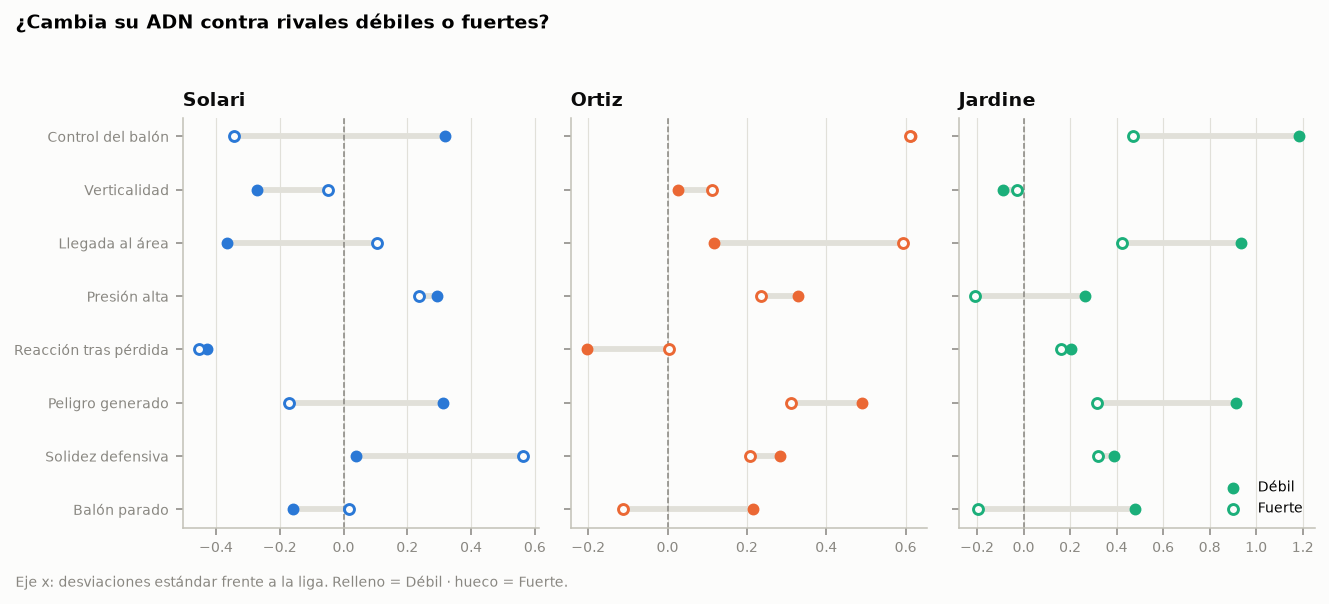
\includegraphics[width=\linewidth]{contexto_rival.png}
\caption{Ajuste al rival: rasgos del ADN contra rivales débiles (relleno) y fuertes (hueco). Jardine es el que más
ajusta su plan según el rival (H3).}
\label{fig:adnRival}
\end{figure}

\subsection{El mapa de técnicos de la Liga MX}
\begin{figure}[H]
\centering
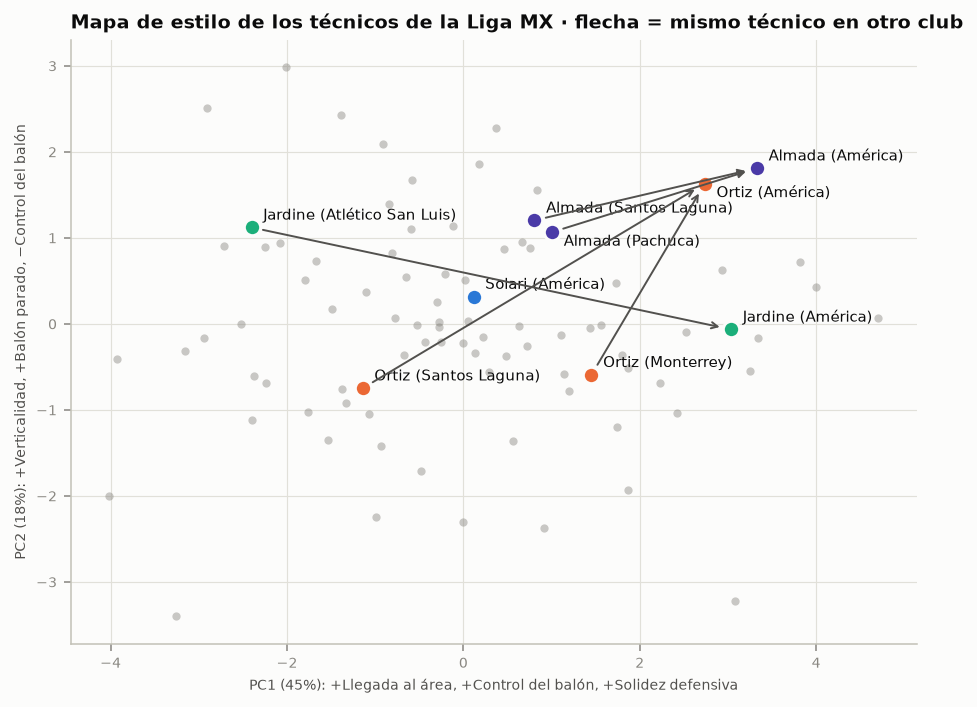
\includegraphics[width=0.9\linewidth]{liga_mapa_estilo.png}
\caption{Mapa de estilo de los técnicos de la Liga MX (PCA de los 8 rasgos). Cada punto es un técnico en un club; las
flechas unen al mismo técnico en dos clubes.}
\label{fig:adnMapa}
\end{figure}

\paragraph{Índice de Encaje (H10).} Es la distancia del ADN de cada técnico-club a la \textbf{identidad histórica del
América}, que es el promedio de sus partidos de 2021--2025. Se expresa de 0 a 100, donde 100 es el más parecido de la
liga. Sirve como lista corta para una contratación: los más cercanos juegan, en promedio, como ha jugado el América.

\begin{table}[H]
\centering
\small
\caption{Índice de Encaje: los 10 técnicos-club de la liga más parecidos a la identidad histórica del América.}
\label{tab:coachFit}
\resizebox{\ifdim\width>\linewidth\linewidth\else\width\fi}{!}{%
\begin{tabular}{lrrr}
\toprule
\textbf{técnico (club)} & \textbf{Índice de Encaje} & \textbf{distancia} & \textbf{partidos} \\
\midrule
Ortiz (América) & 98.6 & 1.1 & 55 \\
Jardine (América) & 97.1 & 1.1 & 91 \\
Renato Paiva (Toluca) & 95.7 & 1.3 & 38 \\
Víctor Vucetich (Monterrey) & 94.3 & 2.0 & 54 \\
Ariel Holan (León) & 92.9 & 2.0 & 38 \\
Ortiz (Monterrey) & 91.4 & 2.1 & 44 \\
Nicolás Larcamón (León) & 90.0 & 2.1 & 39 \\
Miguel Herrera (Tigres UANL) & 88.6 & 2.1 & 62 \\
Vicente Sánchez (Cruz Azul) & 87.1 & 2.2 & 18 \\
Antonio Mohamed (Toluca) & 85.7 & 2.3 & 23 \\
\bottomrule
\end{tabular}}
\end{table}

\subsection{Validación: ¿el ADN reconoce a un técnico en partidos que nunca vio? (H9)}
Un clasificador (regresión logística multinomial) aprende, con toda la liga en la ventana oficial, a reconocer al
técnico a partir de los 8 rasgos de un partido. La etiqueta es el técnico y no el equipo. En la prueba de 2026, el
técnico real está entre los 5 más probables en el \topCincoTest\,\% de los partidos de la liga, frente a un
\azarCinco\,\% por azar (Tabla~\ref{tab:coachTopk}).

\begin{table}[H]
\centering
\small
\caption{¿El ADN reconoce al técnico en partidos que nunca vio? Proporción de partidos de la liga en que el técnico real está entre los k más probables (31 técnicos posibles).}
\label{tab:coachTopk}
\resizebox{\ifdim\width>\linewidth\linewidth\else\width\fi}{!}{%
\begin{tabular}{lrrrrr}
\toprule
\textbf{} & \textbf{top-1} & \textbf{top-3} & \textbf{top-5} & \textbf{partidos} & \textbf{azar top-1} \\
\midrule
validación (Apertura 2025) & 0.05 & 0.11 & 0.22 & 194 & 0.03 \\
prueba (2026) & 0.10 & 0.19 & 0.35 & 155 & 0.03 \\
\bottomrule
\end{tabular}}
\end{table}

\begin{historia}[El estilo sigue al técnico, no a la plantilla]
El modelo nunca vio a Almada dirigir al América: solo lo conocía por su etapa en Pachuca. Aun así, en sus partidos
de 2026 con el América lo ubica en la \textbf{posición mediana \almadaRank{} de 31 técnicos posibles}, y entre los tres
más probables en el \almadaTopTres\,\% de los partidos (Tabla~\ref{tab:coachAmRank}). En promedio, los partidos de
2026 se desplazan del ADN de Jardine hacia el de Almada (Figura~\ref{fig:adnCambio}).

Esto es lo que necesita un club para evaluar candidatos: \textbf{el ADN construido en su club anterior anticipa cómo
jugará en el nuevo}.
\end{historia}

\begin{table}[H]
\centering
\small
\caption{Partidos del América fuera de la ventana oficial: posición del técnico real en el ranking.}
\label{tab:coachAmRank}
\resizebox{\ifdim\width>\linewidth\linewidth\else\width\fi}{!}{%
\begin{tabular}{lrrr}
\toprule
\textbf{técnico · conjunto} & \textbf{partidos} & \textbf{posición mediana} & \textbf{\% en top 3} \\
\midrule
Jardine · test & 19 & 3 & 52.6 \\
Jardine · val & 19 & 2 & 52.6 \\
Almada · test & 9 & 2 & 66.7 \\
\bottomrule
\end{tabular}}
\end{table}

\begin{figure}[H]
\centering
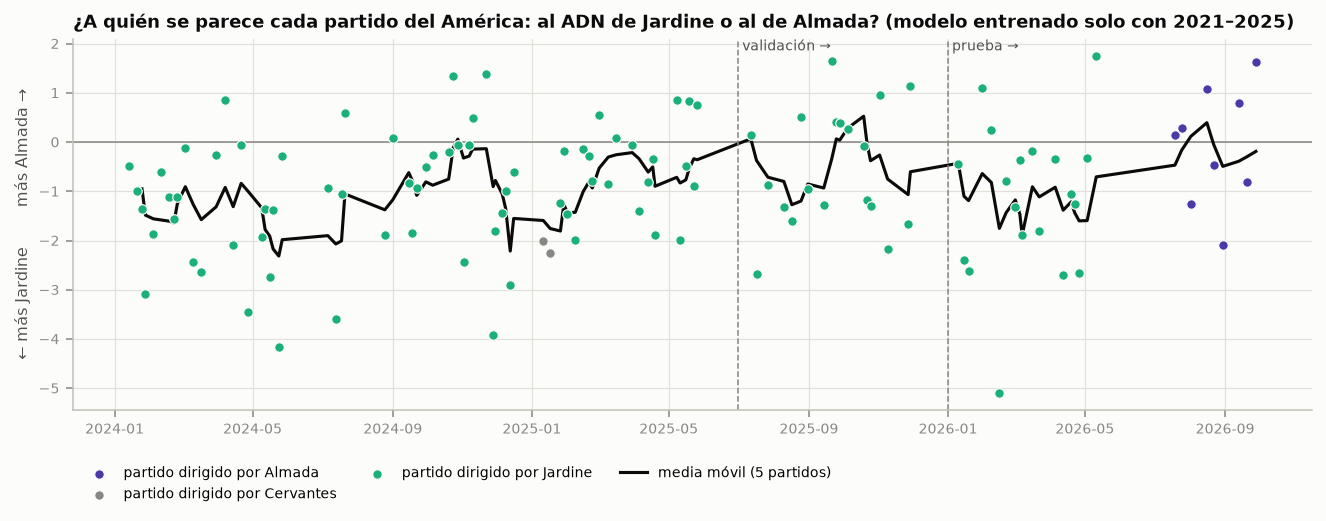
\includegraphics[width=\linewidth]{cambio_tecnico.png}
\caption{Por partido del América: ¿se parece más al ADN de Jardine o al de Almada? Modelo entrenado solo con
2021--2025. La señal por partido es ruidosa; la media móvil muestra el cambio de técnico en 2026.}
\label{fig:adnCambio}
\end{figure}

\subsection{Valor para el club}
\paragraph{Una decisión frecuente y cara.} En la ventana oficial hubo \cambiosTecnico{} cambios de técnico en la Liga
MX, y el \pctCortos\,\% de los periodos duró menos de dos torneos (Tabla~\ref{tab:turnover}). El ADN convierte esa
decisión en una comparación objetiva:
\begin{itemize}
  \item \textbf{Contratación}: ADN e Índice de Encaje de los candidatos frente a la identidad del club.
  \item \textbf{Seguimiento}: ¿el técnico actual mantiene su idea? (Figura~\ref{fig:adnCambio} y monitoreo de drift.)
  \item \textbf{Preparación de partidos}: el ADN del técnico rival.
\end{itemize}

\begin{table}[H]
\centering
\small
\caption{Rotación de técnicos en la Liga MX (ventana oficial, 2021--2025).}
\label{tab:turnover}
\resizebox{\ifdim\width>\linewidth\linewidth\else\width\fi}{!}{%
\begin{tabular}{lr}
\toprule
\textbf{indicador} & \textbf{valor} \\
\midrule
periodos de entrenador & 122.0 \\
equipos & 18.0 \\
cambios de técnico & 104.0 \\
cambios por torneo (liga) & 13.0 \\
partidos por periodo (mediana) & 21.0 \\
\% de periodos de menos de 2 torneos & 69.7 \\
\bottomrule
\end{tabular}}
\end{table}

\paragraph{ROI por escenarios.} Los montos son \textbf{supuestos explícitos}, porque no hay cifras públicas verificadas
de los costos del club (Tabla~\ref{tab:roiAssump}). El beneficio viene de reducir la probabilidad de una contratación
fallida y de ahorrar horas de análisis. En el escenario base el ROI es de \roiBase{} veces el costo anual, y basta con
reducir en un \equilibrioBase\,\% relativo la probabilidad de error para recuperar la inversión. En el conservador, el
ROI es negativo (\roiCons): la herramienta solo se paga si efectivamente mejora las decisiones de técnico.

\begin{table}[H]
\centering
\small
\caption{ROI anual por escenario (montos en millones de pesos; supuestos en la Tabla~\ref{tab:roiAssump}).}
\label{tab:roi}
\resizebox{\ifdim\width>\linewidth\linewidth\else\width\fi}{!}{%
\begin{tabular}{lrrr}
\toprule
\textbf{} & \textbf{Conservador} & \textbf{Base} & \textbf{Optimista} \\
\midrule
ahorro por mejores decisiones de técnico (M MXN) & 0.11 & 1.20 & 5.00 \\
ahorro en horas de análisis (M MXN) & 0.03 & 0.11 & 0.24 \\
beneficio anual (M MXN) & 0.14 & 1.31 & 5.24 \\
costo anual (M MXN) & 0.40 & 0.30 & 0.20 \\
ROI & -0.64 & 3.36 & 25.20 \\
punto de equilibrio (reducción de error) & 0.16 & 0.02 & 0.00 \\
\bottomrule
\end{tabular}}
\end{table}
\begin{table}[H]
\centering
\scriptsize
\caption{Supuestos del modelo de ROI (a validar con el club).}
\label{tab:roiAssump}
\resizebox{\ifdim\width>\linewidth\linewidth\else\width\fi}{!}{%
\begin{tabular}{l r r r p{5.8cm}}
\toprule
\textbf{supuesto} & \textbf{Conservador} & \textbf{Base} & \textbf{Optimista} & \textbf{supuesto} \\
\midrule
costo\_cambio\_tecnico & 15,000,000 & 30,000,000 & 50,000,000 & Costo de cambiar de técnico antes de tiempo: indemnización, salario remanente y nuevo cuerpo técnico. \\
prob\_cambio\_fallido & 0.30 & 0.40 & 0.50 & Probabilidad de que una contratación termine antes de dos torneos (se contrasta con la rotación observada). \\
reduccion\_error & 0.05 & 0.10 & 0.20 & Reducción relativa de esa probabilidad al elegir con el ADN y el Índice de Encaje. \\
decisiones\_por\_anio & 0.50 & 1.00 & 1.00 & Evaluaciones de técnico por año (contratación o renovación). \\
horas\_ahorradas\_partido & 2.00 & 4.00 & 6.00 & Horas de analista ahorradas por partido gracias a la ficha automática. \\
partidos\_por\_anio & 40.00 & 45.00 & 50.00 & Partidos analizados por año (propios y de rivales). \\
costo\_hora\_analista & 400.00 & 600.00 & 800.00 & Costo por hora de un analista. \\
costo\_anual\_herramienta & 400,000 & 300,000 & 200,000 & Costo anual de mantener la herramienta (sin licencias: Python local). \\
\bottomrule
\end{tabular}}
\end{table}

\paragraph{Escalabilidad y activación.}
\begin{itemize}
  \item \textbf{Escalabilidad}: el mismo código perfila a los \nTecnicos{} técnicos de la liga, y cambiar de competición
        (Liga MX Femenil u otra liga con datos StatsBomb) es cambiar un parámetro.
  \item \textbf{Activación}: tarjeta ``ADN del partido'' para la afición (solo agregados) y ficha previa con el ADN del
        técnico rival para el cuerpo técnico.
\end{itemize}

\begin{table}[H]
\centering
\footnotesize
\caption{Veredicto preliminar de hipótesis del EDA con el ADN del entrenador y la partición oficial.}
\label{tab:coachHyp}
\resizebox{\ifdim\width>\linewidth\linewidth\else\width\fi}{!}{%
\begin{tabular}{l p{4.6cm} p{9.2cm}}
\toprule
\textbf{H} & \textbf{hipótesis} & \textbf{evidencia} \\
\midrule
H1 & Cada técnico tiene un ADN distinguible & Top-5 en prueba 35\% frente a 16\% por azar; perfiles del América separados en presión y control \\
H2 & Identidad del club frente a la del técnico & Rasgos de club: Balón parado, Solidez defensiva · del técnico: Llegada al área, Control del balón \\
H3 & Jardine se adapta al rival más que Solari y Ortiz & Ajuste total fuerte -- débil: Solari 2.62, Ortiz 1.45, Jardine 3.15 \\
H9 & El ADN detecta un técnico que nunca vio & Almada en el América: posición mediana 2 de 31 técnicos \\
H10 & El Índice de Encaje ordena a los técnicos de la liga & Top 3: Ortiz (América), Jardine (América), Renato Paiva (Toluca) \\
\bottomrule
\end{tabular}}
\end{table}

% =====================================================================
\section{Implementación: la ficha como producto}\label{sec:implementacion}
% =====================================================================
\subsection{¿Hace falta un \emph{model registry}?}
Un registry completo (versiones, estados de aprobación, despliegue) no se justifica para un equipo pequeño que trabaja
en local: git versiona el código y el pipeline regenera todo. Lo mínimo útil es una \textbf{model card} por modelo:
\texttt{models/<nombre>.joblib} con el pipeline entrenado y \texttt{.json} con la tarea, las variables, los
hiperparámetros, las fechas de entrenamiento, la métrica frente al baseline y el \emph{hash} de la tabla Gold. La regla
de uso: si \texttt{beats\_baseline} es falso, la ficha usa el baseline. Ejemplo:

{\footnotesize\VerbatimInput{tables/card_example.txt}}

\subsection{Scoring en batch y ficha automática}
La etapa \texttt{score} calcula, para cada partido:
\begin{itemize}
  \item el estilo esperado según T1 (o el baseline) frente al observado;
  \item la posición en el mapa de estilo, el tipo de partido y los tres partidos más parecidos (KNN);
  \item la probabilidad del resultado por \textbf{simulación Monte Carlo del xG}: cada tiro es un Bernoulli con
        probabilidad igual a su xG y se simulan 10,000 repeticiones del partido.
\end{itemize}
La etapa \texttt{report} genera una ficha HTML estática (Jinja2 + matplotlib) que lee solo de Gold, de los scores y de
las \emph{model cards}. Secciones:
\begin{enumerate}
  \item contexto;
  \item crónica automática;
  \item el partido en números por criterio (percentil frente a los partidos de entrenamiento);
  \item uso de jugadores;
  \item comparación histórica;
  \item momentos;
  \item balón parado;
  \item proyección (esperado frente a observado y siguiente partido);
  \item monitoreo de drift;
  \item trazabilidad.
\end{enumerate}
Se generaron dos ejemplos: la final de vuelta del Apertura 2024 (Monterrey 1--1, visita) y el partido de fase regular
con mayor dominio territorial (Santos 3--0, field tilt 91\,\%).

\begin{figure}[H]
\centering
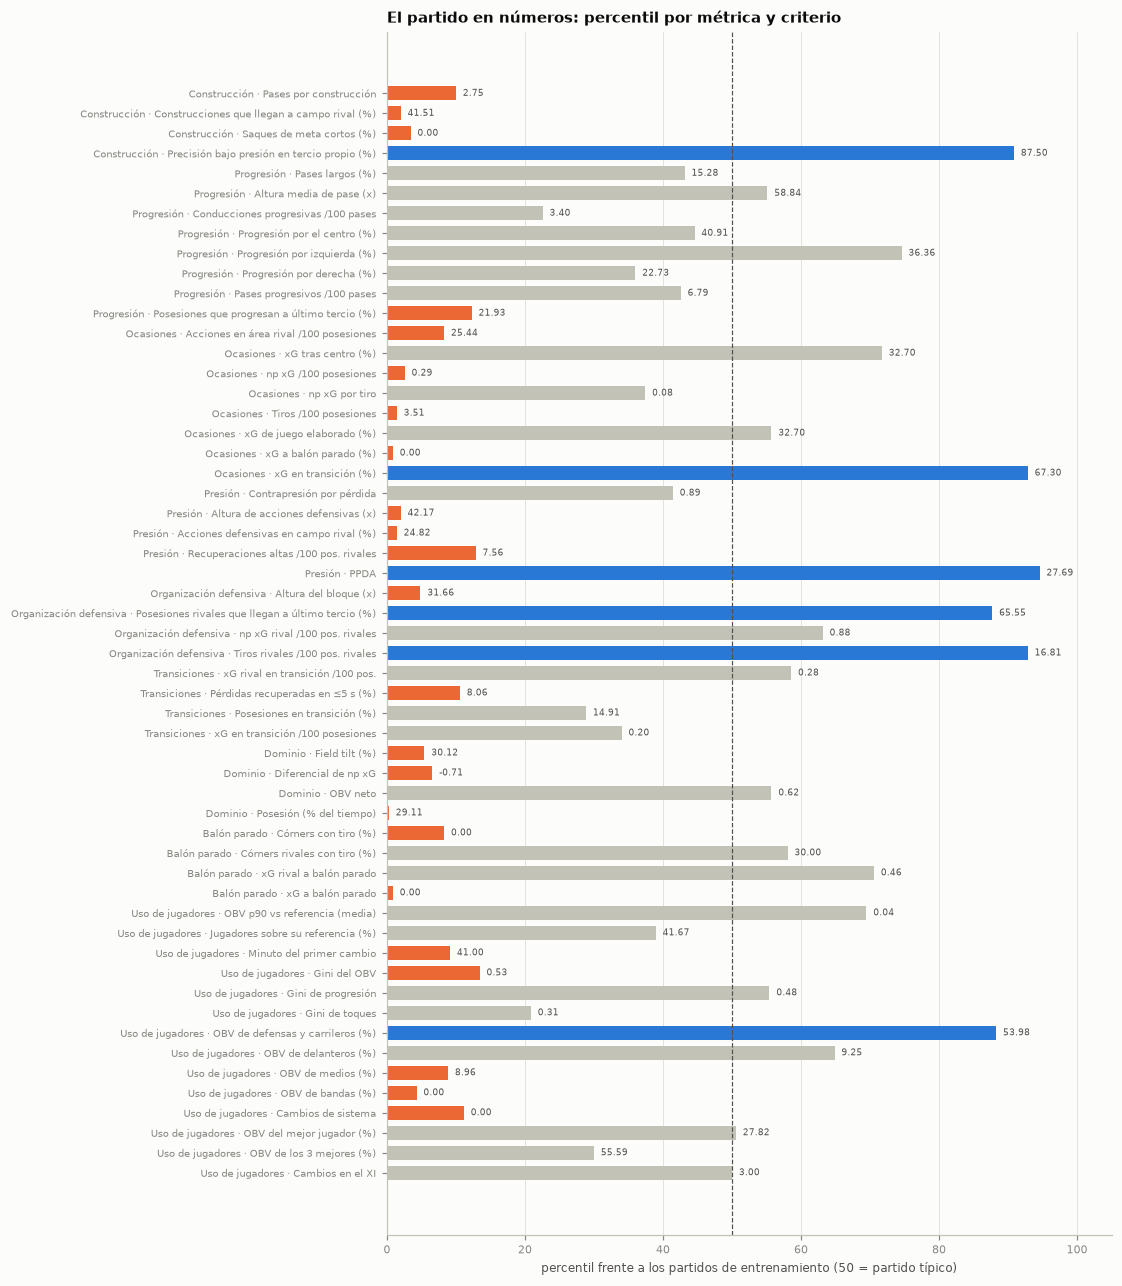
\includegraphics[width=0.85\linewidth]{ficha_percentiles.png}
\caption{Ficha de la final del Apertura 2024: percentil de cada métrica frente a los partidos de entrenamiento (azul: $\geq80$; naranja: $\leq20$).}
\label{fig:fichaPct}
\end{figure}

\begin{historia}[Lo que la ficha cuenta de la final sin haberla visto]
\begin{itemize}
  \item Fue un partido reactivo (tipo 2): la posesión estuvo en el percentil 0 y la presión en campo rival en el 1.
  \item Se defendió abajo y resistió: la precisión bajo presión en la salida estuvo en el percentil 91, y el valor lo
        generaron defensas y carrileros (54\,\% del OBV positivo).
  \item El modelo de contexto esperaba más posesión ($-2.3$ desviaciones estándar) y más presión en campo rival
        ($-2.1$): el plan se desvió de lo habitual.
  \item Con los tiros que hubo, el resultado más probable era la derrota (P = 53\,\%); el empate que dio el título fue,
        según el xG, un resultado favorable.
\end{itemize}
\end{historia}

\begin{figure}[H]
\centering
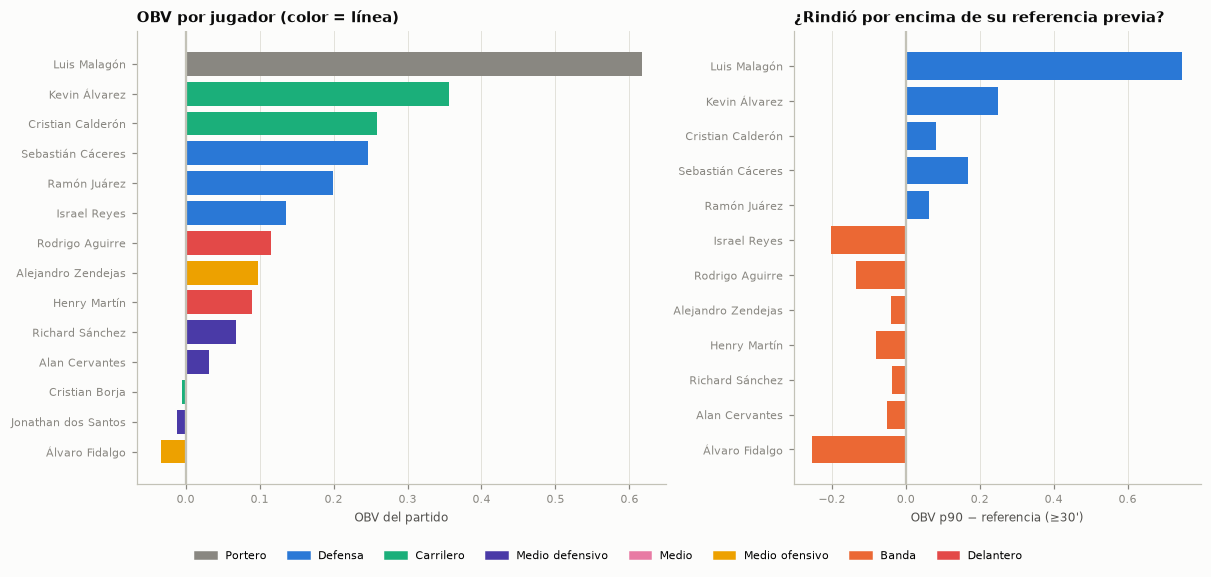
\includegraphics[width=\linewidth]{ficha_players.png}
\caption{Ficha de la final: OBV por jugador (color = línea) y rendimiento frente a la referencia previa de cada jugador.}
\label{fig:fichaPlayers}
\end{figure}

\begin{figure}[H]
\centering
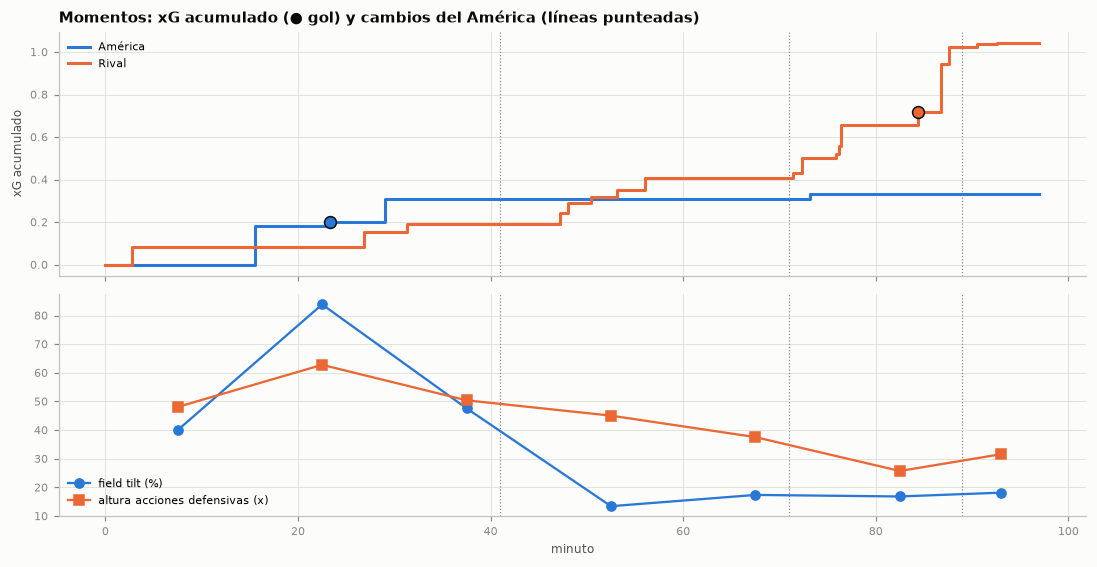
\includegraphics[width=\linewidth]{ficha_timeline.png}
\caption{Ficha de la final: xG acumulado, goles y cambios (arriba); field tilt y altura de las acciones defensivas por
tramo (abajo).}
\label{fig:fichaTimeline}
\end{figure}

\subsection{Monitoreo de \emph{drift}}
El PSI (\emph{Population Stability Index}) compara la distribución reciente de cada variable con la de
entrenamiento. Con ventanas de 10 partidos, el PSI esperado \emph{sin} drift ya ronda 0.4, así que los umbrales clásicos
(0.10 y 0.25) marcarían drift siempre. Por eso los umbrales se calibran por remuestreo: 1,000 muestras de 10 partidos de
entrenamiento dan la distribución nula, y se marca drift moderado por encima del percentil 90 y fuerte por encima del 99
(Tabla~\ref{tab:drift}). Con este criterio, en los últimos 10 partidos (ya con Almada) los pases largos y los
pases progresivos muestran un cambio moderado; ninguna variable llega a fuerte.

\begin{table}[H]
\centering
\small
\caption{Monitoreo de drift: PSI de los últimos 10 partidos frente a entrenamiento, con umbrales calibrados por remuestreo.}
\label{tab:drift}
\resizebox{\ifdim\width>\linewidth\linewidth\else\width\fi}{!}{%
\begin{tabular}{lrrrrrr}
\toprule
\textbf{variable} & \textbf{PSI} & \textbf{p90 nulo} & \textbf{p99 nulo} & \textbf{media train} & \textbf{media reciente} & \textbf{estado} \\
\midrule
Pases largos (\%) & 0.663 & 0.555 & 0.839 & 16.498 & 18.397 & moderado \\
Pases progresivos /100 pases & 0.555 & 0.527 & 0.821 & 6.978 & 7.912 & moderado \\
PPDA & 0.501 & 0.549 & 0.843 & 14.242 & 11.608 & estable \\
np xG rival /100 pos. rivales & 0.488 & 0.555 & 0.889 & 0.809 & 1.233 & estable \\
Altura media de pase (x) & 0.312 & 0.527 & 0.889 & 58.234 & 61.898 & estable \\
Posesiones en transición (\%) & 0.308 & 0.539 & 0.853 & 17.974 & 16.605 & estable \\
Posesión (\% del tiempo) & 0.311 & 0.555 & 0.839 & 53.392 & 58.142 & estable \\
np xG /100 posesiones & 0.244 & 0.488 & 0.839 & 1.370 & 1.393 & estable \\
Field tilt (\%) & 0.176 & 0.527 & 0.839 & 59.175 & 62.280 & estable \\
Acciones defensivas en campo rival (\%) & 0.127 & 0.539 & 0.831 & 41.559 & 43.656 & estable \\
Saques de meta cortos (\%) & 0.112 & 0.556 & 0.783 & 41.071 & 47.353 & estable \\
Altura de acciones defensivas (x) & 0.000 & 0.555 & 0.889 & 53.378 & 54.243 & estable \\
\bottomrule
\end{tabular}}
\end{table}

% =====================================================================
\section{Limitaciones y siguientes pasos}\label{sec:limitaciones}
% =====================================================================
\begin{itemize}
  \item \textbf{Muestra}: 222 partidos es poco para modelos flexibles. Por eso se privilegian modelos regularizados e
        interpretables, y las mejoras sobre el baseline son modestas.
  \item \textbf{Causalidad}: todos los resultados son asociaciones. El efecto del contexto sobre el estilo (T1, T2) no
        separa la decisión propia de la respuesta del rival.
  \item \textbf{Rival}: la fuerza del rival se mide con puntos previos, no con su estilo. Un siguiente paso es
        caracterizar a cada rival con las mismas variables.
  \item \textbf{360}: los datos de 360 están en Silver pero aún no se usan en variables (por ejemplo, pases que rompen
        líneas o presión por compañeros cercanos).
  \item \textbf{Calibración}: las probabilidades de T4 y T5 deben recalibrarse antes de leerse como tales.
  \item \textbf{Siguiente fase}: usar este marco para comparar periodos y entrenadores con las variables núcleo,
        contrastar las hipótesis del EDA y convertir la ficha en la base de la narrativa final.
\end{itemize}

\appendix
% =====================================================================
\section{Supuestos del marco}\label{app:assumptions}
\begin{table}[H]
\centering
\footnotesize
\caption{Supuestos y umbrales del marco (\texttt{framework.ASSUMPTIONS}).}
\label{tab:assumptions}
\resizebox{\ifdim\width>\linewidth\linewidth\else\width\fi}{!}{%
\begin{tabular}{l p{9cm}}
\toprule
\textbf{supuesto} & \textbf{valor} \\
\midrule
pitch & (120, 80) \\
third\_limits & (40, 80) \\
lane\_limits & (26.666666666666668, 53.333333333333336) \\
box & \{'x\_min': 102, 'y\_min': 18, 'y\_max': 62\} \\
danger\_zone & \{'x\_min': 90, 'y\_min': 18, 'y\_max': 62\} \\
offensive\_sequence\_min\_passes & 3 \\
build\_up\_start\_x\_max & 40 \\
progression\_from\_x\_max & 60 \\
transition\_window\_s & 15 \\
counterpress\_window\_s & 5 \\
press\_high\_x & 60 \\
press\_mid\_x & 40 \\
ppda\_def\_zone\_x & 48 \\
ppda\_opp\_pass\_x\_max & 72 \\
progressive\_min\_gain & 0.25 \\
progressive\_end\_x\_min & 48 \\
set\_piece\_throw\_in\_x\_min & 80 \\
minute\_bins & [0, 15, 30, 45, 60, 75, 90, 200] \\
minute\_labels & ['0-15', '15-30', '30-45+', '45-60', '60-75', '75-90', '90+'] \\
player\_min\_minutes & 30 \\
player\_reference\_window & 10 \\
rival\_strength\_window & 17 \\
sub\_window\_min & 15 \\
\bottomrule
\end{tabular}}
\end{table}

\section{Catálogo de variables}\label{app:catalog}
{\scriptsize
\begin{longtable}{p{3.4cm} p{3.3cm} p{2.2cm} p{5.2cm} p{2.6cm}}
\caption{Catálogo de variables por partido (\texttt{features.FEATURES} y \texttt{PLAYER\_FEATURES}).}\label{tab:catalog}\\
\toprule
\textbf{variable} & \textbf{etiqueta} & \textbf{criterio} & \textbf{definición} & \textbf{dirección} \\
\midrule
\endfirsthead
\toprule
\textbf{variable} & \textbf{etiqueta} & \textbf{criterio} & \textbf{definición} & \textbf{dirección} \\
\midrule
\endhead
\bottomrule
\endfoot
gk\_short\_goal\_kick\_pct & Saques de meta cortos (\%) & Construcción & \% de saques de meta cortos (longitud < 32 yd) & + = salida corta \\
buildup\_passes\_per\_seq & Pases por construcción & Construcción & Pases medios por posesión de construcción (inicio x<40) & + = elaboración \\
buildup\_success\_pct & Construcciones que llegan a campo rival (\%) & Construcción & \% de construcciones que llegan a campo rival (x$\geq$60) & + = mejor salida \\
press\_resistance\_own\_third & Precisión bajo presión en tercio propio (\%) & Construcción & Precisión de pase bajo presión en tercio propio & + = resiste presión \\
prog\_passes\_per100 & Pases progresivos /100 pases & Progresión & Pases progresivos por 100 pases & + = más vertical \\
prog\_carries\_per100 & Conducciones progresivas /100 pases & Progresión & Conducciones progresivas por 100 pases & + = progresa conduciendo \\
prog\_lane\_left\_pct & Progresión por izquierda (\%) & Progresión & \% de pases progresivos que terminan en carril izquierdo & carril \\
prog\_lane\_center\_pct & Progresión por el centro (\%) & Progresión & \% de pases progresivos que terminan en carril central & carril \\
prog\_lane\_right\_pct & Progresión por derecha (\%) & Progresión & \% de pases progresivos que terminan en carril derecho & carril \\
progression\_rate & Posesiones que progresan a último tercio (\%) & Progresión & \% de posesiones que cruzan de x<60 a x$\geq$80 & + = progresa más \\
pass\_x\_mean & Altura media de pase (x) & Progresión & Altura media de los pases propios (x) & + = juega más arriba \\
long\_pass\_pct & Pases largos (\%) & Progresión & \% de pases largos ($\geq$ 32 yd) en juego abierto & + = más directo \\
np\_xg\_per100poss & np xG /100 posesiones & Ocasiones & np xG por 100 posesiones propias & + = más peligro \\
np\_xg\_per\_shot & np xG por tiro & Ocasiones & np xG por tiro & + = mejores ocasiones \\
shots\_per100poss & Tiros /100 posesiones & Ocasiones & Tiros por 100 posesiones propias & + = más volumen \\
box\_touches\_per100poss & Acciones en área rival /100 posesiones & Ocasiones & Acciones en el área rival por 100 posesiones & + = pisa más el área \\
xg\_share\_open\_play & xG de juego elaborado (\%) & Ocasiones & \% del xG propio en posesiones de juego abierto (no transición, no BP) & origen \\
xg\_share\_transition & xG en transición (\%) & Ocasiones & \% del xG propio en transiciones & origen \\
xg\_share\_set\_piece & xG a balón parado (\%) & Ocasiones & \% del xG propio en balón parado & origen \\
cross\_xg\_share & xG tras centro (\%) & Ocasiones & \% del xG propio de tiros asistidos con centro & + = juego por centros \\
ppda & PPDA & Presión & Pases rivales de juego abierto (x$\leq$72) por entrada/intercepción/falta propia (x$\geq$48) & -- = presión más intensa \\
def\_action\_x\_mean & Altura de acciones defensivas (x) & Presión & Altura media de las acciones defensivas propias (x) & + = defiende más arriba \\
high\_press\_pct & Acciones defensivas en campo rival (\%) & Presión & \% de acciones defensivas en campo rival (x$\geq$60) & + = presión alta \\
high\_regains\_per100opp & Recuperaciones altas /100 pos. rivales & Presión & Recuperaciones que inician posesión en x$\geq$60 por 100 posesiones rivales & + = roba arriba \\
counterpress\_per\_loss & Contrapresión por pérdida & Presión & Acciones de contrapresión por pérdida en juego & + = reacción tras pérdida \\
opp\_np\_xg\_per100poss & np xG rival /100 pos. rivales & Organización defensiva & np xG rival por 100 posesiones rivales & -- = defiende mejor \\
opp\_shots\_per100poss & Tiros rivales /100 pos. rivales & Organización defensiva & Tiros rivales por 100 posesiones rivales & -- = concede menos \\
opp\_f3\_entry\_pct & Posesiones rivales que llegan a último tercio (\%) & Organización defensiva & \% de posesiones rivales que llegan a x$\geq$80 & -- = bloque más sólido \\
block\_x\_mean & Altura del bloque (x) & Organización defensiva & Altura media de duelos, intercepciones, bloqueos y despejes & + = bloque alto \\
transition\_poss\_pct & Posesiones en transición (\%) & Transiciones & \% de posesiones propias que son transición ofensiva & + = juego de transición \\
transition\_xg\_per100poss & xG en transición /100 posesiones & Transiciones & xG en transición por 100 posesiones propias & + = castiga al contragolpe \\
opp\_transition\_xg\_per100poss & xG rival en transición /100 pos. & Transiciones & xG rival en transición por 100 posesiones rivales & -- = controla transición defensiva \\
quick\_regain\_pct & Pérdidas recuperadas en $\leq$5 s (\%) & Transiciones & \% de pérdidas recuperadas en $\leq$ 5 s & + = contrapresión efectiva \\
possession\_time\_pct & Posesión (\% del tiempo) & Dominio & \% del tiempo de posesión (duración de posesiones) & + = más balón \\
field\_tilt & Field tilt (\%) & Dominio & Pases propios en último tercio / pases de ambos en su último tercio & + = domina territorio \\
obv\_net & OBV neto & Dominio & OBV propio -- OBV rival & + = domina en valor \\
np\_xg\_diff & Diferencial de np xG & Dominio & np xG propio -- np xG rival & + = domina en ocasiones \\
sp\_xg & xG a balón parado & Balón parado & xG propio en balón parado & + = peligro a balón parado \\
opp\_sp\_xg & xG rival a balón parado & Balón parado & xG rival en balón parado & -- = defiende bien el BP \\
corner\_shot\_pct & Córners con tiro (\%) & Balón parado & \% de córners propios que terminan en tiro & + = córners efectivos \\
opp\_corner\_shot\_pct & Córners rivales con tiro (\%) & Balón parado & \% de córners rivales que terminan en tiro & -- = defiende bien córners \\
gini\_obv & Gini del OBV & Uso de jugadores & Gini del OBV ($\geq$0) entre jugadores propios & + = juego concentrado \\
gini\_touches & Gini de toques & Uso de jugadores & Gini de toques entre jugadores de campo & + = balón concentrado \\
gini\_prog & Gini de progresión & Uso de jugadores & Gini de acciones progresivas & + = progresión concentrada \\
top1\_obv\_share & OBV del mejor jugador (\%) & Uso de jugadores & \% del OBV positivo del mejor jugador & + = depende de uno \\
top3\_obv\_share & OBV de los 3 mejores (\%) & Uso de jugadores & \% del OBV positivo de los 3 mejores & + = depende de pocos \\
obv\_share\_def & OBV de defensas y carrileros (\%) & Uso de jugadores & \% del OBV positivo generado por defensas y carrileros & línea \\
obv\_share\_mid & OBV de medios (\%) & Uso de jugadores & \% del OBV positivo generado por medios & línea \\
obv\_share\_wide & OBV de bandas (\%) & Uso de jugadores & \% del OBV positivo generado por bandas & línea \\
obv\_share\_fwd & OBV de delanteros (\%) & Uso de jugadores & \% del OBV positivo generado por delanteros & línea \\
boost\_pct & Jugadores sobre su referencia (\%) & Uso de jugadores & \% de jugadores ($\geq$30') por encima de su OBV p90 de referencia previa & + = el sistema los potencia \\
boost\_mean & OBV p90 vs referencia (media) & Uso de jugadores & Media del OBV p90 -- referencia previa, jugadores $\geq$30' & + = el sistema los potencia \\
xi\_rotation & Cambios en el XI & Uso de jugadores & Titulares distintos respecto al partido anterior & + = rota más \\
tactical\_shifts & Cambios de sistema & Uso de jugadores & Cambios de sistema en el partido (Tactical Shift) & + = ajusta en vivo \\
first\_sub\_minute & Minuto del primer cambio & Uso de jugadores & Minuto del primer cambio & -- = interviene antes \\
\end{longtable}
}

\section{Evaluación completa de variables}\label{app:varEval}
{\scriptsize
\begin{longtable}{p{4.2cm} p{2.3cm} rrrrrrc p{2.9cm}}
\caption{Evaluación de las variables como criterios. Fiab.\ = fiabilidad intra-partido (Spearman-Brown); ICC = ICC(1) con dos tiempos; lag-1 = autocorrelación entre partidos; $R^2$ ctx = variación explicada por localía, rival y fase; máx $|\rho|$ = redundancia; $\rho$ xG = validez frente al diferencial de np xG.}\label{tab:varEval}\\
\toprule
\textbf{variable} & \textbf{criterio} & \textbf{fiab.} & \textbf{ICC} & \textbf{lag-1} & \textbf{$R^2$ ctx} & \textbf{máx $|\rho|$} & \textbf{$\rho$ xG} & \textbf{núcleo} & \textbf{motivo} \\
\midrule
\endfirsthead
\toprule
\textbf{variable} & \textbf{criterio} & \textbf{fiab.} & \textbf{ICC} & \textbf{lag-1} & \textbf{$R^2$ ctx} & \textbf{máx $|\rho|$} & \textbf{$\rho$ xG} & \textbf{núcleo} & \textbf{motivo} \\
\midrule
\endhead
\bottomrule
\endfoot
xG a balón parado & Balón parado & 0.22 & 0.08 & -0.09 & 0.07 & 0.68 & 0.54 & no & fiabilidad baja \\
xG rival a balón parado & Balón parado & 0.09 & 0.09 & -0.03 & 0.02 & 0.71 & -0.48 & no & fiabilidad baja \\
Córners con tiro (\%) & Balón parado & 0.10 & 0.07 & -0.11 & 0.05 & 0.38 & 0.17 & no & fiabilidad baja \\
Córners rivales con tiro (\%) & Balón parado & 0.07 & 0.02 & 0.05 & 0.05 & 0.49 & -0.28 & no & fiabilidad baja \\
Precisión bajo presión en tercio propio (\%) & Construcción & 0.19 & 0.11 & 0.20 & 0.00 & 0.24 & 0.24 & no & fiabilidad baja \\
Saques de meta cortos (\%) & Construcción & 0.45 & 0.31 & 0.14 & 0.06 & 0.46 & 0.17 & sí &  \\
Pases por construcción & Construcción & 0.40 & 0.22 & 0.05 & 0.09 & 0.60 & 0.28 & sí &  \\
Construcciones que llegan a campo rival (\%) & Construcción & 0.37 & 0.21 & 0.21 & 0.08 & 0.67 & 0.22 & sí &  \\
Field tilt (\%) & Dominio & 0.55 & 0.40 & -0.00 & 0.09 & 0.76 & 0.33 & no & VIF 10.1 \\
Posesión (\% del tiempo) & Dominio & 0.40 & 0.27 & 0.07 & 0.10 & 0.75 & 0.27 & sí &  \\
np xG por tiro & Ocasiones & 0.23 & 0.13 & 0.14 & 0.00 & 0.69 & 0.56 & no & fiabilidad baja \\
xG de juego elaborado (\%) & Ocasiones & 0.00 & -0.02 & 0.08 & 0.02 & 0.47 & -0.05 & no & fiabilidad baja \\
xG en transición (\%) & Ocasiones & 0.24 & 0.15 & 0.00 & 0.05 & 0.79 & 0.07 & no & fiabilidad baja \\
xG a balón parado (\%) & Ocasiones & 0.19 & 0.09 & -0.08 & 0.02 & 0.68 & 0.04 & no & fiabilidad baja \\
xG tras centro (\%) & Ocasiones & 0.09 & 0.02 & 0.04 & 0.03 & 0.26 & 0.13 & no & fiabilidad baja \\
np xG /100 posesiones & Ocasiones & 0.30 & 0.19 & 0.07 & 0.08 & 0.82 & 0.82 & sí &  \\
Tiros /100 posesiones & Ocasiones & 0.36 & 0.17 & 0.03 & 0.16 & 0.72 & 0.60 & sí &  \\
Acciones en área rival /100 posesiones & Ocasiones & 0.46 & 0.29 & 0.10 & 0.06 & 0.62 & 0.52 & sí &  \\
np xG rival /100 pos. rivales & Organización defensiva & 0.09 & 0.03 & -0.09 & 0.01 & 0.71 & -0.57 & no & fiabilidad baja \\
Tiros rivales /100 pos. rivales & Organización defensiva & 0.09 & 0.10 & -0.11 & 0.04 & 0.64 & -0.45 & no & fiabilidad baja \\
Posesiones rivales que llegan a último tercio (\%) & Organización defensiva & 0.38 & 0.22 & 0.14 & 0.09 & 0.80 & -0.26 & sí &  \\
Altura del bloque (x) & Organización defensiva & 0.37 & 0.24 & 0.07 & 0.06 & 0.85 & 0.30 & sí &  \\
Acciones defensivas en campo rival (\%) & Presión & 0.43 & 0.25 & -0.03 & 0.09 & 0.96 & 0.32 & no & redundante con def\_action\_x\_mean \\
Recuperaciones altas /100 pos. rivales & Presión & 0.24 & 0.15 & 0.08 & 0.09 & 0.64 & 0.26 & no & fiabilidad baja \\
PPDA & Presión & 0.50 & 0.14 & 0.22 & 0.07 & 0.41 & -0.06 & sí &  \\
Altura de acciones defensivas (x) & Presión & 0.44 & 0.28 & 0.00 & 0.08 & 0.96 & 0.35 & sí &  \\
Contrapresión por pérdida & Presión & 0.32 & 0.19 & 0.12 & 0.01 & 0.26 & 0.07 & sí &  \\
Progresión por izquierda (\%) & Progresión & 0.10 & 0.07 & 0.07 & 0.02 & 0.48 & -0.08 & no & fiabilidad baja \\
Progresión por derecha (\%) & Progresión & 0.24 & 0.14 & 0.04 & 0.03 & 0.54 & -0.01 & no & fiabilidad baja \\
Pases progresivos /100 pases & Progresión & 0.36 & 0.14 & 0.01 & 0.03 & 0.39 & 0.23 & sí &  \\
Conducciones progresivas /100 pases & Progresión & 0.30 & 0.14 & 0.13 & 0.04 & 0.36 & 0.19 & sí &  \\
Progresión por el centro (\%) & Progresión & 0.38 & 0.22 & -0.01 & 0.01 & 0.54 & 0.13 & sí &  \\
Posesiones que progresan a último tercio (\%) & Progresión & 0.45 & 0.26 & 0.21 & 0.03 & 0.67 & 0.25 & sí &  \\
Altura media de pase (x) & Progresión & 0.47 & 0.31 & 0.12 & 0.03 & 0.76 & 0.25 & sí &  \\
Pases largos (\%) & Progresión & 0.63 & 0.45 & 0.34 & 0.01 & 0.41 & -0.21 & sí &  \\
xG rival en transición /100 pos. & Transiciones & 0.13 & -0.03 & -0.03 & 0.01 & 0.58 & -0.37 & no & fiabilidad baja \\
Pérdidas recuperadas en $\leq$5 s (\%) & Transiciones & -- & -- & -0.04 & 0.03 & 0.28 & 0.14 & no & sin estabilidad (lag-1 $\leq$ 0) \\
Posesiones en transición (\%) & Transiciones & 0.33 & 0.19 & 0.04 & 0.04 & 0.59 & 0.33 & sí &  \\
xG en transición /100 posesiones & Transiciones & 0.30 & 0.11 & 0.10 & 0.06 & 0.79 & 0.48 & sí &  \\
Gini del OBV & Uso de jugadores & -- & -- & -0.00 & 0.03 & 0.95 & -0.19 & no & sin estabilidad (lag-1 $\leq$ 0) \\
OBV de los 3 mejores (\%) & Uso de jugadores & -- & -- & -0.04 & 0.04 & 0.95 & -0.19 & no & sin estabilidad (lag-1 $\leq$ 0) \\
OBV de defensas y carrileros (\%) & Uso de jugadores & -- & -- & -0.02 & 0.02 & 0.40 & -0.28 & no & sin estabilidad (lag-1 $\leq$ 0) \\
OBV de bandas (\%) & Uso de jugadores & -- & -- & -0.11 & 0.06 & 0.36 & 0.34 & no & sin estabilidad (lag-1 $\leq$ 0) \\
OBV de delanteros (\%) & Uso de jugadores & -- & -- & -0.06 & 0.02 & 0.34 & 0.24 & no & sin estabilidad (lag-1 $\leq$ 0) \\
Gini de toques & Uso de jugadores & -- & -- & 0.08 & 0.03 & 0.41 & 0.16 & sí &  \\
Gini de progresión & Uso de jugadores & -- & -- & 0.05 & 0.03 & 0.41 & -0.04 & sí &  \\
OBV del mejor jugador (\%) & Uso de jugadores & -- & -- & 0.07 & 0.03 & 0.82 & -0.18 & sí &  \\
OBV de medios (\%) & Uso de jugadores & -- & -- & 0.04 & 0.01 & 0.27 & 0.12 & sí &  \\
Jugadores sobre su referencia (\%) & Uso de jugadores & -- & -- & 0.11 & 0.06 & 0.67 & 0.32 & sí &  \\
OBV p90 vs referencia (media) & Uso de jugadores & -- & -- & 0.14 & 0.07 & 0.67 & 0.26 & sí &  \\
Cambios en el XI & Uso de jugadores & -- & -- & 0.25 & 0.10 & 0.22 & 0.04 & sí &  \\
Cambios de sistema & Uso de jugadores & -- & -- & 0.17 & 0.01 & 0.22 & -0.06 & sí &  \\
Minuto del primer cambio & Uso de jugadores & -- & -- & 0.02 & 0.03 & 0.34 & 0.20 & sí &  \\
\end{longtable}
}

\section{Model cards}\label{app:cards}
{\scriptsize
\begin{longtable}{lrrrrrrr}
\caption{Resumen de las model cards: métrica en la prueba temporal frente al mejor baseline.}\label{tab:cards}\\
\toprule
\textbf{model card} & \textbf{tarea} & \textbf{modelo} & \textbf{MAE} & \textbf{MAE baseline} & \textbf{ROC-AUC} & \textbf{F1 macro} & \textbf{supera} \\
\midrule
\endfirsthead
\toprule
\textbf{model card} & \textbf{tarea} & \textbf{modelo} & \textbf{MAE} & \textbf{MAE baseline} & \textbf{ROC-AUC} & \textbf{F1 macro} & \textbf{supera} \\
\midrule
\endhead
\bottomrule
\endfoot
T1\_def\_action\_x\_mean & T1 & Árbol & 4.963 & 4.671 & -- & -- & no \\
T1\_field\_tilt & T1 & KNN & 13.318 & 14.244 & -- & -- & sí \\
T1\_gk\_short\_goal\_kick\_pct & T1 & LASSO & 23.581 & 24.038 & -- & -- & sí \\
T1\_high\_press\_pct & T1 & Árbol & 7.245 & 7.112 & -- & -- & no \\
T1\_long\_pass\_pct & T1 & LASSO & 2.135 & 2.000 & -- & -- & no \\
T1\_np\_xg\_per100poss & T1 & Ridge & 0.546 & 0.460 & -- & -- & no \\
T1\_opp\_np\_xg\_per100poss & T1 & KNN & 0.464 & 0.479 & -- & -- & sí \\
T1\_pass\_x\_mean & T1 & Ridge & 4.377 & 4.339 & -- & -- & no \\
T1\_possession\_time\_pct & T1 & Árbol & 7.696 & 8.476 & -- & -- & sí \\
T1\_ppda & T1 & Ridge & 5.248 & 4.918 & -- & -- & no \\
T1\_prog\_passes\_per100 & T1 & KNN & 1.418 & 1.360 & -- & -- & no \\
T1\_transition\_poss\_pct & T1 & Ridge & 4.034 & 3.711 & -- & -- & no \\
T2\_def\_action\_x\_mean & T2 & Ridge & 9.014 & 9.305 & -- & -- & sí \\
T2\_field\_tilt & T2 & Ridge & 21.004 & 22.863 & -- & -- & sí \\
T2\_high\_press\_pct & T2 & Ridge & 13.065 & 13.334 & -- & -- & sí \\
T2\_long\_pass\_pct & T2 & Ridge & 5.428 & 5.455 & -- & -- & sí \\
T2\_pass\_x\_mean & T2 & Ridge & 7.677 & 8.108 & -- & -- & sí \\
T2\_possession\_time\_pct & T2 & Ridge & 14.481 & 15.130 & -- & -- & sí \\
T3\_np\_xg\_diff & T3 & LASSO & 0.581 & 0.705 & -- & -- & sí \\
T3\_obv\_net & T3 & LASSO & 1.371 & 1.371 & -- & -- & no \\
T3b\_result & T3b & Logística softmax & -- & -- & -- & 0.310 & sí \\
T4\_shot & T4 & Logística & -- & -- & 0.719 & -- & sí \\
T5\_contra\_shot & T5\_contra & Logística & -- & -- & 0.710 & -- & sí \\
T5\_favor\_shot & T5\_favor & Logística & -- & -- & 0.683 & -- & sí \\
T6\_d\_field\_tilt & T6 & Ridge & 22.967 & 22.810 & -- & -- & no \\
T6\_d\_np\_xg\_diff & T6 & Ridge & 0.322 & 0.317 & -- & -- & no \\
T6\_d\_obv\_net & T6 & Ridge & 0.704 & 0.712 & -- & -- & sí \\
T7\_boost\_mean & T7 & Ridge & 0.093 & 0.100 & -- & -- & sí \\
T7\_gini\_prog & T7 & Árbol & 0.065 & 0.065 & -- & -- & sí \\
T7\_gini\_touches & T7 & Ridge & 0.030 & 0.030 & -- & -- & no \\
T7\_top3\_obv\_share & T7 & Árbol & 8.126 & 8.569 & -- & -- & sí \\
U1U2\_style\_space & U1/U2 & -- & -- & -- & -- & -- & -- \\
U3\_player\_roles & U3 & -- & -- & -- & -- & -- & -- \\
\end{longtable}
}

\section{Tablas complementarias}
\begin{table}[H]
\centering
\footnotesize
\caption{U1 -- Cargas de las componentes principales.}
\label{tab:u1Load}
\resizebox{\ifdim\width>\linewidth\linewidth\else\width\fi}{!}{%
\begin{tabular}{lrrrrr}
\toprule
\textbf{variable} & \textbf{PC1} & \textbf{PC2} & \textbf{PC3} & \textbf{PC4} & \textbf{PC5} \\
\midrule
Posesión (\% del tiempo) & 0.36 & 0.01 & -0.21 & 0.22 & -0.32 \\
Field tilt (\%) & 0.43 & -0.05 & -0.14 & 0.11 & -0.00 \\
PPDA & -0.21 & -0.46 & 0.14 & -0.16 & 0.41 \\
Altura de acciones defensivas (x) & 0.40 & 0.11 & -0.08 & -0.27 & 0.30 \\
Acciones defensivas en campo rival (\%) & 0.38 & 0.11 & -0.09 & -0.31 & 0.34 \\
Altura media de pase (x) & 0.38 & 0.11 & -0.01 & 0.28 & 0.07 \\
Pases progresivos /100 pases & 0.08 & 0.35 & 0.65 & 0.29 & -0.14 \\
Pases largos (\%) & -0.18 & 0.57 & 0.01 & -0.10 & 0.09 \\
Saques de meta cortos (\%) & 0.18 & -0.45 & -0.04 & 0.03 & -0.42 \\
Posesiones en transición (\%) & 0.28 & -0.07 & 0.29 & -0.01 & 0.27 \\
np xG /100 posesiones & 0.16 & -0.29 & 0.60 & -0.02 & 0.02 \\
np xG rival /100 pos. rivales & -0.11 & -0.10 & -0.18 & 0.76 & 0.49 \\
\bottomrule
\end{tabular}}
\end{table}
\begin{table}[H]
\centering
\small
\caption{U1 -- Varianza explicada por las componentes retenidas (PCA ajustado con train).}
\label{tab:u1}
\resizebox{\ifdim\width>\linewidth\linewidth\else\width\fi}{!}{%
\begin{tabular}{lrr}
\toprule
\textbf{} & \textbf{varianza} & \textbf{acumulada} \\
\midrule
PC1 & 0.370 & 0.370 \\
PC2 & 0.126 & 0.495 \\
PC3 & 0.107 & 0.602 \\
PC4 & 0.088 & 0.690 \\
PC5 & 0.075 & 0.765 \\
\bottomrule
\end{tabular}}
\end{table}

\end{document}
